\chapter{Practice of Change}
\label{chap:practice}

\textit{In theory there is no difference between theory and practice...} - Benjamin Brewster \cite{brewster1882} \\


The Media Lab has deep roots in Constructionism --- learning through doing --- beginning with Media Lab co-founding faculty member Seymour Papert who defined constructionism in his 1987 National Science Foundation proposal,``Constructionism: A New Opportunity for Elementary Science Education'' \cite{papert1986constructionism}. It is fitting that almost everything that I have learned, I have learned through doing things and being mentored along the way. This chapter represents three decades of learning through doing.

I have learned by experience that learning through doing can be hard at first, especially if you have very little learning before you start, for you may lack the frameworks that traditional educational models explicitly convey. What you learn by doing depends on what you happen to be doing, and so may lack the coherence that traditional discipline-based systems provide. It can be difficult to build that coherent view, and it's easy to go wrong if you don't know the extent of what you don't know: a lack of discipline and an absence of disciplines can lead to attempts to ``boil the ocean'' in pursuit of a single unified theory of everything.

However, over the years one's model of the world may start to come together, as one's influence and trust in many different networks mature; as one's ability to translate and connect ideas across networks and disciplines increases; and as opportunities and problems present themselves from odd but often useful perspectives.

My seven years as the Media Lab's director have put my natural affinity for constructionism to the test, for now I was expected to lead one of the most highly respected research centers in the world. But most academic institutions are not particularly comfortable with ``learning by doing'' or the community-based, antidisciplinary approach I have long advocated. In order to provide such an environment at relative scale --- about eight hundred people in our extended community --- required learning how to hop back and forth across the boundary that separates traditional institutional mechanisms and the ``heterotopia'' that has made the Lab so highly regarded externally, and so cherished by MIT and its community members. 

In this chapter we will explore this boundary.

\section{The Antidisciplinary Approach}
\label{antidisciplinaryapproach}

\marginpar{Being antidisciplinary faces the the same challenges that I did growing up: how do you manage being interested in learning about everything without the structure and the boundaries traditionally imposed? For both individuals and organizations, the best approach is passion-based constructionism.}An antidisciplinary approach is necessary to advance the paradigm shift that we require. The Media Lab is both the institute where the concept arose and the best example I know of an antidisciplinary organization.\footnote{Portions of the following sections about the Media Lab are based on a journal article and a talk that I gave at the Innovation Research Interchange induction ceremony in 2017, when I was the recipient of the IRI Medal. The talk was later published in the journal, \textit{Research-Technology Management} \cite{ito2017antidisciplinary}. It describes how the Media Lab works and provides my opinion about its trajectory and principles.}

Being antidisciplinary faces the the same challenges that I did growing up: how do you manage being interested in learning about everything without the structure and the boundaries traditionally imposed? For both individuals and organizations, the best approach is passion-based constructionism.

\subsection{Joining the Media Lab}

When I joined the Media Lab as its director in 2011, I had one way of doing things, and the Media Lab had another. 

I was transitioning from the world of Internet entrepreneurship and open-source governance to academia. At first, it didn't make sense that I, with my background as a scrappy entrepreneur, could fit in at a huge academic institution like MIT. But the Media Lab was different. It is antidisciplinary --- not opposed to disciplines, but explicitly seeking out ideas and research agendas that work across disciplines. The Media Lab has always favored research that falls into the white space between disciplines. It allows students and researchers the freedom to explore --- and to fail. And it has produced some groundbreaking inventions that its corporate members have gone on to commercialize with great success. Those differences, provide important lessons for all kinds of organizations --- research labs, companies, even academic institutions --- that are being challenged to adapt to the tidal waves of change that we're all facing now. 

\subsection{The History of the MIT Media Lab}

The Media Lab is somewhat peculiar, even for a highly diversified university like MIT. That peculiarity arises from the Lab's history. It was founded 32 years ago by former MIT president Jerome Wiesner and a young faculty member named Nicholas Negroponte. Wiesner had stepped down as president several years earlier but wanted to continue working in areas about which he was passionate, which included bringing the arts and sciences together at MIT. Negroponte, who was promoting a vision of a digital future that included a CAD system on everyone's desktop, was working on computer-aided design in the Architecture Machine Group in MIT's School of Architecture and Planning. Together they created the Media Lab.

And when they created it, they did something you can only do when your partner is the former president of MIT: They broke a bunch of rules. Typically in universities, you have labs and you have academic programs, and they tend to work like church and state in a healthy or unhealthy balance. The academic program offers classes to students and grants degrees. Labs, on the other hand, focus on raising funds to conduct specific research aimed at real-world impact. The Media Lab is both. It has its own academic program --- the Program in Media Arts within MIT's School of Architecture and Planning --- and it is also a research lab. 

The other unique aspect of the Media Lab is its funding model. When the Lab opened, approximately 80 percent of MIT's funding came from government sources and 20 percent came from private sources. The Media Lab was the exact opposite, with 80 percent of its money coming from corporate sources. This was partly a result of Wiesner's history. As science advisor to John F. Kennedy, he was sent to Japan to help that country rebuild its technology and research infrastructure. As a result, many in the Japanese business world felt a real debt to Wiesner. At the time Wiesner and Negroponte were planning the Media Lab, these companies had money to spend. So much of the money for launching the Media Lab came from the CEOs and chairmen of Japanese electronics firms. In fact, the Media Lab was even criticized for selling secrets to the Japanese \cite{MITDealW66:online}.

The way the lab handles its corporate support is also atypical for academia. Funds from corporate members do not support directed research, but rather go into one Lab-wide fund, and any IP (intellectual property) resulting from Lab research is available to be shared among all the corporate members. In the past, members could choose among different consortia to join based on their research interests, but today there is just one consortium for all members.

Currently, the total lab budget is about \$75 million, the majority from the consortium and some from government and other non-IP-generating research grants. As director, I distribute consortium funds to 25 research groups, which are working on everything from synthetic neurobiology to the future of opera. Each research group is made up of students and faculty members. Crucially, the research groups have almost full license to spend the money on whatever they want, at their discretion. This enables them to explore, fail, learn, and explore some more.

\subsection{How the Media Lab Works}

This structure has a couple of major consequences for the way the Media Lab works. 

First, it helps to create a strong sense of community. In a typical lab, if you're a faculty researcher, you write a grant proposal, your students work with you,and together you deliver the required results. Such a system makes it difficult for people from different labs or departments to work with one another. It can even make it difficult for the funding companies to work with one another. Everybody's working on their own grants, and the IP generated by that research must be protected from all the other groups. But at the Media Lab, the consortium owns the IP, so there's no barrier to collaboration. Twice a year, hundreds of people from our member organizations --- from LEGO to Lockheed Martin to governments --- come to the lab to learn about the current research. Amazingly, even companies that are normally fierce competitors, such as LG, Samsung, Toshiba, and Google, join together in this unique member community.

The pooling of IP gives us the freedom to fund things that others wouldn't. The member companies aren't supporting us so that we'll help them do better what they're already doing. They support us because we might do something they would never have thought to do on their own. That makes working in the white spaces core to the Media Lab's ``business model.''

We try very hard to find interesting areas of research that would be impossible to fund in other departments or labs because they are in between disciplines or are too risky and strange. In fact, we try to exit areas when they become mainstream.

\subsection{Accounting}

When I joined the Media Lab, it was recovering from the 2008 downturn in the economy. What I didn't know was that the Lab had during the 2001 downtown also suffered from a serious accounting error that had led to an overestimation of its financial resources: MIT and the Media Lab had been recognizing all revenue for a three year contract in the year the contract was signed, even when payment was not yet due. This made it look like the Lab had much more money than it really did. Because new contracts kept coming in, no one noticed until the downturn. Once the downturn hit it became clear that the Lab had been spending well ahead of revenue. In late 2001, this led to significant layoffs. 

While all this took place many years before I arrived, the Lab was still traumatized by this event, and across MIT still had a reputation for being poorly managed.

When I joined, I was told that the books were balanced and that the debt had been paid off. After my first year when the surplus from that year's income disappeared, I investigated and discovered that there was a hidden liability of millions of dollars somewhere in the accounting system of MIT.

After substantial effort in trying to fix the finances and accounting system, I reached out to a colleague of mine from several previous companies where we worked together. Barak Berkowitz had been the president of Six Apart and OmniSky, a public company, and had been an investment manager with me. He came in to help me fix the accounting system.

We discovered that the accounting system was set up in a way that made our finances completely opaque to both the Media Lab and central MIT finance. There was no consistent way to track the most basic things. How much money does the Lab have available to spend? How much money do we need next year? Did we make or lose money last year? The new Vice President of Finance, Israel Ruiz, had come from industry and understood how complicated and broken the accounting system was.

We spent many months trying to sort through what was actually going on in the accounting system. At the same time, we redesigned the financial reports to look more like a company with a balance sheet and a profit and loss statement. Originally, the Lab was set up as if it were a single research project that had been going on for thirty years and had no prospect of ending. Instead of the central MIT administration and the Media trying to hide things from each other, we made our system as transparent and representative of the facts as we could, and we agreed on a consistent way to judge the financial condition of the Lab.

We never were able to get to the bottom of the obscure liabilities that the Media Lab was thought to have with the central finance department so we agreed to start fresh, and zero the accounts from the day I took the job at the Media Lab.

Once the accounting system was fixed, we were able to build many systems, thanks to Berkowitz, the finance team, the human resources team, and all of the staff. From an operations perspective, the Media Lab was now running as much like a business as possible at MIT.

For the Media Lab to be both the instrument of change and an example of the theory of change it espouses, some very traditional structures need to be in place. Disruption needs a firm platform to stand on.

\subsection{Membership Model and Growth}

One of the first things that I did when I joined the Media Lab was change the label for our funders from ``sponsors'' to ``members''. I wanted to make it clear that the companies were members of our community and to be respected as colleagues, not our bosses telling us what to do or ``dumb money'' that stands back from community. While the Media Lab was never as directed as most labs, my predecessor, Frank Moss, appeared to be focused a bit more on commercialization to support the Consortium's member companies, which could have an inhibiting effect on the freedom that the Lab originally had enjoyed \cite{FrankMos10:online}. This was in part a response to the difficult financial situation that the Lab was in at the time after the 2008 downturn. I tried to make it clear that while we worked with our companies and listened to them, the Lab was exploring areas that the companies don't yet know they would be interested in.

I also initiated a price increase because the Consortium membership, \$200,000 a year, had not been increased for fifteen years. We decided to increase it to \$250,000 a year. Our initial presentation of this change was poorly communicated and we had significant pushback from companies. We got together, regrouped, tweaked the contract and reintroduced the change with much greater success. 

While this process damaged our relationship with some members and we lost a significant number of them, it turned out to be critical for building a tighter relationship with the companies that stayed. In addition the companies that left were the ones that did not believe they were getting value they wanted out of the Lab. We quickly replaced them with companies that were excited and more engaged with the Lab. This is consistent with the Lab's model of treating funders as engaged members of a unique research community. Today the average member spends well over \$300k a year with the Lab when you include incremental funding they provide to projects that especially interest them.

The consortium model described in the paper \autoref{antidisciplinaryapproach} has continued to thrive. The continuing robustness of the financial markets clearly have had a supporting effect, but our membership numbers and overall revenue has increased every year over the seven years that I've been here. (See \autoref{mlpandl}.)

\begin{figure}[h]
 \centering
 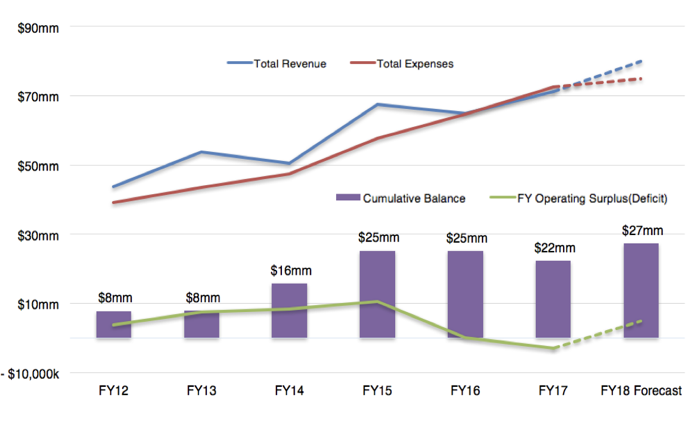
\includegraphics[width=1\textwidth]{pictures/mlpandl.png}
 \caption{Media Lab Consolidated P\&L}
 \label{mlpandl}
\end{figure}

Recently, we presented these numbers at a meeting of entire Lab. I reported that we had 475 full time staff including the students, and nearly 800 people in our ecosystem if we include the part-time undergraduate researchers in addition to the Masters and Ph.D. students. I reported these numbers with pride.

Later that evening when I was leaving the Lab, a long-time researcher who has a very good sensibility about the Media Lab culture approached me and asked, ``When are we too big?'' I mentioned that we had thirty tenure track slots and that we currently had 26 groups and that maybe that was a good limit. As I said that, I realized that some groups had become quite large. The researcher also mentioned that it is virtually impossible to know eight hundred people's names, much less to know those people well.

\marginpar{One significant question for me is, ``What is the right size for the Media Lab?'' How do we decide what to do and what not to do? How do we increase quality over quantity? How do we determine quality?}I realized that while I espouse the limits of growth and warn about the danger of focusing on growth, I had been doing it myself. Initially, fixing the accounting system and bringing in cash was essential to build up the health of the organization. But now we were healthy. Maybe more than enough is too much.

One significant question for me is, ``What is the right size for the Media Lab?'' How do we decide what to do and what not to do? How do we increase quality over quantity? How do we determine quality?

While some believe in a somewhat hierarchical model of tenure track faculty deciding everything, I believe that the dynamics of the community determine the quality and the flourishing of the system.

We were, in fact, facing one of the core dilemmas in the age of connected technology: How to scale community?

\subsection{Community}

When I arrived at the Media Lab, women had represented about twenty percent of the student population for as far back as we could see. The Visiting Committee, an external committee of a variety of experts from inside and outside of MIT that audits the Media Lab's overall performance every two years, had noted for the last four years that this gender diversity was unacceptable. Additionally, the number of minorities at the Media Lab was also unacceptable.

I had heard from former Media Lab graduates that they didn't recommend the Media Lab to prospective female applicants because it didn't feel safe for women. I realized that this wasn't an issue of just trying to get our faculty to admit more women -- they were in fact admitted in line with the percentage of female applicants. I realized that  to change the pipeline we needed not just to alter our communications about our culture, but change the reality of our culture, and of our community. While disciplines are based around topics, communities and cultures are based on the actual people in them.

I spent several years trying harder, but the numbers only moved slightly. Then we hired Monica Orta as a director of diversity. Her sole focus was on increasing the diversity of students applying to the Media Lab. But her first task was to actually make the Media Lab safer and more welcoming to minorities and women. We worked together to address issues as quickly as we could. For example, unacceptable behavior on mailing lists was immediately dealt with. Harassment and other issues were dealt with quickly and firmly. After some member company visitors talked to students in gender and racially insensitive ways, I opened the next member meeting with a message to the thousand attendees that they are members of our community, and we have zero tolerance for any member who does not support our community's values.

With Monica's help, now nearly fifty percent of incoming students are women. 

\begin{figure}[h]
 \centering
 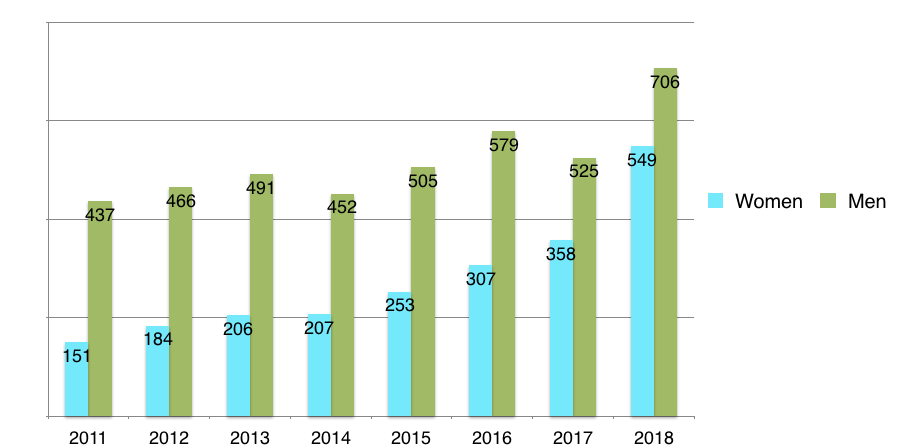
\includegraphics[width=1\textwidth]{pictures/mlgender.png}
 \caption{Master’s Applications by Gender}
 \label{mlgender}
\end{figure}

Unfortunately, our racial and ethic diversity has not improved as much as the gender diversity, but it is improving slightly. (See \autoref{mldiversity}.)

Our most recent faculty hire, Danielle Wood, is an African-American woman who has publicly vowed to make diversity an important part of her work.

\begin{figure}[h]
 \centering
 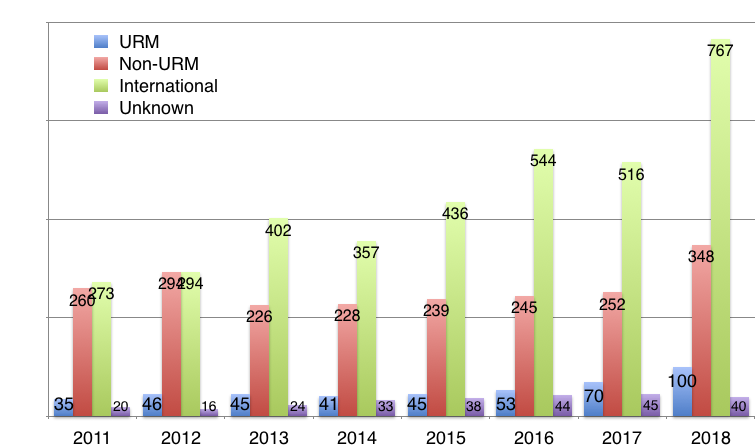
\includegraphics[width=1\textwidth]{pictures/2018mldiversity.png}
 \caption{Master’s Applications by Race/Ethnicity}
 \label{mldiversity}
\end{figure}

Diversity among the faculty hires has been more difficult than with students. The faculty do not turn over as quickly and since we add them one at a time, it is harder to implement policy.

This is now one of my most important areas of focus.

The total student application numbers of students have increased significantly and our response to faculty searches is also strong. (See \autoref{mladmissions}.) This is encouraging news, but I do worry that as we become competitive and able to hire stronger students and faculty who have significant competing offers, we could lose the Salon des Refusés feeling that has so characterized the Media Lab.

\begin{figure}[h]
 \centering
 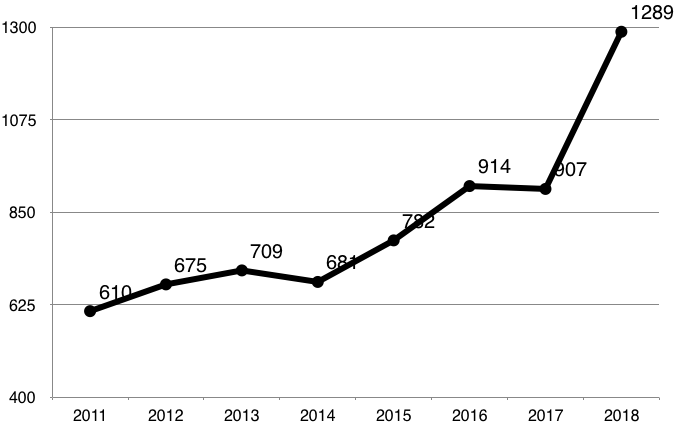
\includegraphics[width=1\textwidth]{pictures/2018mladmissions.png}
 \caption{Total Number of Applications (Master's and PhD)}
 \label{mladmissions}
\end{figure}

\subsection{The Media Lab Mindset}

The companies that interact with the Media Lab are seeking that discovery sensibility; they're looking for an exploration rather than a problem-solving kind of thinking. In a book I recently coauthored with Jeff Howe, \emph{Whiplash} \cite{ito2016whiplash}, I tried to capture the core principles driving the Media Lab. \emph{Whiplash} grew out of almost five years of discussion as my colleagues and I worked through the collision between the Media Lab's peculiar DNA and the DNA I brought from the Internet world. In those discussions, we developed a set of principles, iterated on over multiple faculty meetings, by asking two questions: What are the principles that define the Media Lab? and What are the principles that drive innovation on the Internet?

The Internet brought many changes, but among the most important was the recognition that the Newtonian laws that had governed how companies operate now turned out to be local ordinances that only worked in certain cases. Everything moved faster, everything was hyper-connected. Some models didn't survive. Some models thrived. Some companies --- some big companies --- were able to survive this transition, and a whole new set of players entered the scene. But the old rules were gone, and a new set of guiding principles emerged. We began to see agile, bottom-up systems outperforming those built around more rigid top-down authority. Organizations with a more creative vision and culture were more likely to succeed than those with elaborate, well-documented plans. The ever-decreasing cost of innovation allowed for --- in fact necessitated --- taking more risk. These are the principles that we talk about in \emph{Whiplash} (See \autoref{principles}). And they are the principles that drive much of what the Media Lab is doing now.

\begin{table}[H]
\centering
\caption{Innovation principles for the age of the Internet}
\label{principles}
\begin{tabular}{| L{3cm} | L{7cm} |}
\hline
Emergence \textit{over} Authority & Complex, bottom-up systems beat out top-down authority.       \\ \hline
Pull \textit{over} Push  & Resources and innovation should be pulled from the edges rather than controlled from the center.  \\ \hline
Compasses \textit{over} Maps  & Detailed plans (maps) become less valuable than vision, values, and culture.     \\ \hline
Risk \textit{over} Safety  & With the cost of innovation coming down, the focus should be on taking smart risks rather than seeking safety. \\ \hline
Disobedience \textit{over} Compliance & Agile, effective innovators will question authority and think independently.     \\ \hline
Practice \textit{over} Theory  & Focus less on theory and more on learning by doing.        \\ \hline
Diversity \textit{over} Expertise & A nontraditional team approach will be more productive than the abilities of any one individual.  \\ \hline
Resilience \textit{over} Strength & Resilience will come from failure, especially with complex, adaptive systems.    \\ \hline
Systems \textit{over} Objects  & Everything is connected to everything else; to succeed, you must understand the full ecosystem.  \\ \hline
Learning \textit{over} Education & Fixed educational systems must be replaced with lifelong learning.      \\ \hline
\end{tabular}
\end{table}

\subsection{Permissionless Innovation}

The first thing the Internet did was drive down the cost of innovation. In the early 1990s, we were running a magazine website for Asahi Shimbun (a newspaper) in Japan off of a server in our bathroom. One day the server's fan failed, and then the hard disk failed, and then we were taking turns blowing on the hard disk until somebody could get a new fan.

In the Internet world, we called this ``best effort'':  you couldn't guarantee your hard disk would never fail, but your promised that you would do your very best if it did. A telephone company trying to create an Internet service provider would probably have spent millions of dollars building an infrastructure. What we did took a bathroom and a couple thousand dollars.

\marginpar{Lowering the cost of innovation doesn't just change what it costs to do something. It also changes how you do it, as well as what you can think about doing.}This is permissionless innovation. We didn't ask if we could do this, and we didn't check what the rules were. We just did what we could do. For the first time, a handful of students could actually compete with a telco. That was enabled by the openness of the ecosystem: everything we ran on those servers was free and open-source software. This kind of activity forces competition by driving the price down to what's functionally zero compared to where it was before. When you add Moore's Law to that, you get very low cost technology that increases in power without increasing in price. Network these powerful computers and it creates an explosion of free and open-source software, which in turn lowers the cost of innovation.

Lowering the cost of innovation doesn't just change what it costs to do something. It also changes how you do it, as well as what you can think about doing. In the old days, we had the cable companies and the telephone companies trying to do multimedia over set-top boxes or kiosks, such as the Minitel system in France. These systems cost hundreds of millions --- if not billions --- of dollars because every company had to do it all: the lines, switches, computers, database, software, and content. This kind of complexity required a tremendously detailed plan with lots of dependencies that made the plan tremendously complex to implement correctly. I call this \ac{MBA}-driven innovation. Its opposite is engineer-driven innovation.

When you're in an \ac{MBA}-driven innovation system, you have money, you have permission, you have jobs, you have a system of authority that generates the capital required to do something. The talent chases the money because you need so much money to even get started. With engineer-driven innovation, you have a bunch of college students (or dropouts) running around making things, and venture capitalists chasing them, trying to get in on a good deal. The money chases the talent. It's a very different dynamic.

For some kinds of projects, where the cost of what you want to do is substantial, spending some percentage of that cost to minimize risk makes sense --- building roads or designing airplanes, for example. But if the project is inexpensive --- say only a couple hundred thousand dollars --- and if the cost of failure is just the failure of that thing, the permission costs can exceed the actual costs. I had a company for which I was trying to get an investment of \$600,000; the potential funders spent about \$3 million deciding not to do it. If they had just given me the \$600,000, I could have shown them whether it worked or not, and if it worked, they'd have made some money. Permission granting can be an expensive process that tries to guess whether something will work instead of finding out for real by building it. If the permission process has a negative outcome, the money spent on the process provides only a theory of what might have happened. If an attempt to build something fails, you will have learned something that will help the next project succeed. In general, my rule of thumb is that of the cost of assessing risk and providing permission exceeds the cost of trying it, why not try it? 

\marginpar{No one asks me as director for permission to do a project, but twice a year everyone is required to do a demo of the things they've been working on so the entire community can learn from one another's advances and setbacks.}Additionally, if the experience you might gain is valuable, consider that too. That's why at the Media Lab we think of every failure as an opportunity to capture information. In considering whether to pursue a project, we ask if the information we might get is worth the investment. No one asks me as director for permission to do a project, but twice a year everyone is required to do a demo of the things they've been working on so the entire community can learn from one another's advances and setbacks. This constant interaction among the researchers and the companies is perhaps the main value of joining the Media Lab.

The key is having the right facilities and equipment to keep things inexpensive. At the Media Lab, when there's a conversation and someone hits on an idea, they're in the shop making it by the afternoon, and by the end of the week, there's a photo of it with a video, a rough demo, and all the files needed for somebody else to recreate it. 

But, permission-less innovation is only feasible when the costs are low enough. The Internet and digital revolution have dramatically lowered those costs, but it helps to have the backing of a research center that can provide material support, as well as the community and culture that encourages antidisciplinary innovation in the white spaces. Permission-lessness is free as in speech, not always as in beer.

\subsection{Motivations of Researchers}

The increasingly competitive offers from businesses especially in computer science are depleting research universities of talent. Large companies and even non-profits hire researchers for millions of dollars and provide them with labs equipped more lavishly than university labs. We've seen this particularly acutely at the Media Lab's cryptocurrencies project. Many researchers are quitting academia to join fintech (financial technology) startups or to start their own currencies or digital securities offerings.

While the community at MIT and the Media Lab is of course still able to attract talent, in some fields it has become more of a challenge. An important part of the Media Lab's response has been to help advance one of the counter paradigms to why we assume people take jobs.

We generally have assumed that job applicants are rational, self-interested actors looking to enter into a new contract that compensates them for their work by paying them money. But academics traditionally have been motivated less by money than by other values, including intrinsic values such as the joy of teaching, discovery, and collegiality. The Principles in Awareness class that I describe in \autoref{section:awareness} takes this a step further, helping students find the intrinsic rewards that matter to them. Intrinsic rewards I believe are the most robust of the motivators. But that requires discovering what truly makes one happy.\footnote{In our awareness class, we use the term intrinsic motivation vs extrinsic motivation to differentiate between personal motivations and the motivations that are caused directly by external pressure, stress or a need to please. We work on trying to direct our values and motivations to those that emerge from within. However, it is important to note that even intrinsic motivation must be nurtured and supported, and is therefore social. I do not believe the intrinsic motivation as a completely solitary effect exists. \cite{ryan2000self}.}

Without necessarily announcing it as such, the Media Lab makes a similar offer to potential community members: this is a place rich in intrinsic values and goals such as the excitement of learning in the white spaces, the joy of community, and the ability to contribute to the intrinsic values of others outside of the community: you can build something that will make people healthier, improve the planet, provoke someone's curiosity, and bring delight.

\marginpar{While I am interested in trying to understand how to ``scale'' awareness, the idea is almost a contradiction. Many commercial awareness applications and programs have lost much of the core essence of the idea.}The Lab is in the fortunate position of being able to make both sorts of offers to those thinking of joining, for our community includes businesses as well as researchers. For, much as I am committed to paying attention to the intrinsic motivators of those around me, spaces for open innovation such as the Lab should not be sheltered enclaves. Researchers need to be part of the bustling world around them so that their work addresses real needs and so that work can be adopted and have an effect. That, too, is a boundary that needs to be made permeable, and not just research centers like the Media Lab.

While I am interested in trying to understand how to ``scale'' awareness, the idea is almost a contradiction. Many commercial awareness applications and programs have lost much of the core essence of the idea. They may contribute to relaxation and some appreciation of intrinsic motivations, but efforts like our class are nearly impossible to do at scale without missing the point.

I believe that understanding intrinsic and extrinsic motivators and how we can manage communities to strengthen healthy versions of both is a key piece, if not \emph{the} key piece, of improving our institutions as well as society.

\subsection{Leadership}

I often describe my role at the Media Lab as a custodian or a gardener: I am focused on providing nourishment, pruning, and cultivating the community to try to increase its flourishing. While I try to have a vision and a strategy, I aim at supporting the community, not pushing it. I try to be a participant and not just a director. I try to be decisive but inclusive. Instead of trying to provide a crisp and definitive mission for the Media Lab, my job is to manage a vibrant ecosystem of groups, each with different goals and sensibilities, somehow managing to interact with one another to improve the flourishing of the entire ecosystem --- more akin to a rain forest than the Starship Enterprise.

I led \ac{CC} the same way, for, like the Media Lab, it had very technical components, an existing structure, and a mission-oriented community composed of committed people that mainly needed support and an occasional bit of fine-tuning.

\subsection{The Next Generation}

I am increasingly less focused on the scaling of the Lab itself and more interested in scaling what I have learned by transferring my experience to the next generation of leaders and community organizers. Many of the Lab's students and faculty are building communities and it is my great pleasure and mission to support their growth.

It is my hope that the ideas, stories, and learnings in this dissertation might contribute to their success.

\section{Antidisciplinarianism at Work}

The Media Lab is able to keep moving across disciplines because we don't define ourselves by a specific technology or field; we define ourselves by a point of view, a way of doing things, a sensibility. 

Back in the late 1980s and 1990s, we were focused on personal computing, interfaces, and displays. We continue to do those things, but we moved from them into email and networks, and later into big data and social physics. Here are some examples of the antidisciplinarian work currently underway at the Lab. 

\subsection{Bioengineering at the Media Lab}

Thirty years, ago, when I would give talks about the Internet, the newspaper reporters would fall asleep when I tried to explain that their business was going to change. Nicholas Negroponte said in the 1990s that newspapers would be delivered over the Internet, and everybody laughed at him. I feel the same way when I talk about bioengineering these days, because people think of biology as a hospital, medical, pharma thing --- just like people thought the Internet as an information processing thing. Bio is the new digital in the way it will change the world.

Bioengineering will break out of its discipline to reshape things a long way from the medical field. For example, Sorona is a polyester-like material that's created using plant matter. It uses a synthetic microbe to spark the transformation. It's about 30 percent more efficient and much more ecological to manufacture than polyester, and is starting to compete very well against it. 

But Sorona is a product of industrial R\&D; it cost hundreds of millions of dollars and took years and years of research to create it. That kind of large-scale industrial R\&D is starting to change. For example, we're beginning to understand genome bricks, the building blocks that make up DNA chains. There are now efforts to categorize each set of bricks, identifying what each one does. That kind of modular approach makes genetic engineering look more and more like a computer programming language: you can assemble the bricks, stick them into bacteria or yeast, reboot them, and get them to do a variety of things, such as act as sensors or manufacture chemicals. There are Media Lab groups looking for specific compounds, and building genes around them to do things like trigger wireless systems. They're building circuits where the electronic components are living organic material.

Work with genome bricks is progressing rapidly because of the digital side of the interdisciplinary white space it occupies. In the early 2000s, it cost billions of dollars to sequence a genome. It now costs thousands of dollars, and that cost is dropping much faster than Moore's Law would predict. Professor Joe Jacobson, a Media Lab faculty member, helped create a way to print and assemble genes on a semiconductor, which significantly reduces the error rate, increases the speed, and lowers the cost compared to doing it by hand. All of these developments are driving innovation by diminishing its cost. Bioengineering innovation, like digital innovation and hardware innovation before it, is going to start pushing to the edges because it already exists between some edges.

In fact, it's already started happening. Shortly after I started at the Media Lab, I was involved in a project to use recombinant DNA to design a bacterium to create violacein \cite{bolton2014biohackers}, a naturally occurring violet pigment with antibacterial, antifungal and antitumor properties. Currently, violacein costs about \$300,000 a gram \cite{violacei33:online}. Scholars identified a pathway to create violacein and published the gene sequences --- the genome bricks for this pathway. BioBricks are genome bricks that comply to the standardized International Genetically Engineered Machine community. \cite{anderson2010bglbricks}. A Media Lab graduate and his company created a kit with these BioBricks with guidelines on how to design a plasmid with the m. My team and I designed the requisite bacterium online in an open lab book, opening the research out to the Internet. 

Then we used BioBrick vials to assemble the gene, and got some decommissioned hardware from MIT to do the transformation and insert the plasmids into the bacteria. We rebooted the bacteria and fed them, and we could see the nice purple of the violacin in the petri dishes, the signal things were working. We uploaded photos of the results, so that they could be shared with hundreds of other people doing the same thing, along with our lab books, so we could compare our processes with those of other people to see who could design the best violacein factory. Incidentally, we did this at my house --- I didn't realize I was breaking a Cambridge ordinance by doing recombinant DNA work in our home without a Biosafety Level 2 wet lab. But that's what happens when research within a white space needs a physical space to be realized.

Something that would have been done in the labs of one single big pharma company was crowdsourced by an informal band of citizen scientists and kids hacking the genome of a bacteria in their homes. This was almost five years ago.

The trend is growing. MIT sponsors an international genetically engineered machines competition. A crowd of high school and college kids --- about 7,000 of them --- come together every year to share the genetically engineered machines they've created. Some of them are silly, like E. coli that makes dog poo smell like winter mints. Others are a little bit more useful, such as materials that may help us identify land mines using bacterial bio sensors \cite{ELECTRACE2014iGem}. 

Yes, I know: What could go wrong? But you can't put this genie back in the bottle. With the invention of the stunningly easy and low-cost CRISPR gene-editing technique, this capability will be in your high school student's garage any day now. Given the pace of change, having people come together across disciplinary boundaries to talk about the implications of these antidisciplinary technologies is extremely important. Government agencies and academic institutions realize this, at least at some level. Edward You, the Supervisory Special Agent in the FBI's Weapons of Mass Destruction Directorate, Biological Countermeasures Unit, did an amazing thing along these lines. At his encouragement, the FBI convened two or three times all the international biohacking labs. He told them, ``We did it wrong with the Internet. We turned all the hackers against us. This is going to be much more dangerous. This could be much worse. We need your help. You need to be on our side to protect the world from existential threats of rogue or accidental biological mistakes.'' 

Most of the kids I work with are on board with that. The Media Lab is a very big part of the biosafety standards work, and a lot of the bioengineering work we do addresses safety. Certainly, one of the most terrifying things I can think of is an extinction event triggered by a mistake some high school kid made in her garage, but I also think the kids who are doing this are thinking more about safety and protecting the world than any of the kids I grew up with on the Internet. That's a hopeful development.

\subsection{The MIT Knowledge Futures Group}
\label{MITPress}

Whether we are talking about the future of disciplines, or the sharing and creation of knowledge, academic publishing is a key function and institution that needs to be transformed. As a board member of the MIT Press and through my collaborations with them, I believe that new models of academic publishing are viable and essential.

We are working actively on open access publishing, copyright, new structures for peer review, as well as new ways of publishing, sharing and communicating online --- and also through print, face to face meetings, and communities. \footnote{At a recent MIT Press management board meeting May, 2018, we had a discussion of preprint servers. These are websites where many people have begun to post academic papers before they are published. Some authors, in particular tenured researchers for whom traditional publication and credentialing is less important, are publishing exclusively to preprint servers and not submitting to journals. The number of preprint servers and their services have proliferated. Some servers have features that allow reviewers to leave comments directly on the preprint servers and some link to both publications of the paper and reviews of the paper. It is still early days, but it appears to be an emergent form of peer review. While it is unclear how many of the authors are reading the reviews and how much influence the reviews will carry, John Inglis, MIT Press board member and Executive Director of Cold Spring Harbor Laboratory Press shared that there are informal peer review groups that are forming ``in the wild'' and that journals in his field have begun to reference some of these informal reviews \cite{mitpressboard2018}.

While the exact structure that this informal peer review will take is still to be understood and designed, the publishers, authors and reviewers are clearly ready to experiment.}

To that end, the Media Lab and the MIT Press are working together on a new group. The following is a proposal draft by Amy Brand (director of the MIT Press) and me. \\

\begin{quote}
\emph{The MIT \ac{KFG} is a new joint initiative of the MIT Press and the MIT Media Lab. PFG's mission is to transform research publishing from a closed, sequential process, into an open, community-driven one, by incubating and deploying open source publishing technologies. The partnership is the first of its kind between an established publisher and a world-class academic lab devoted to the design of future-facing technologies.}

\textbf{Rationale}

In order for mission driven academic publishers to flourish into the future, it is imperative that we establish our own innovation pathways. Developing open source alternatives to the stranglehold that a small handful of commercial entities now maintain on not only the markets for research information, but also on academic reputation systems, publishing technologies, and digital innovation will be of clear benefit to the research community and the reading public alike. The same can be said for the publication of content from many other domains such as news, law, and industry research. Each domain is often isolated to a small number of corporations whose ownership of the content influences the systems built around said data. We believe universities must assert greater ownership and influence over the ecosystem for the publication of all knowledge given how critical it is to our core mission of knowledge creation and diffusion.
 
\textbf{Objective}

The \ac{KFG} will serve as a test kitchen, incubator, and a staging platform for the development and launch of open source publishing technologies, infrastructure, and aligned open access publications, staffed jointly by the Press and the Media Lab. The open source approach not only reduces the precarious dependency that most non-profit academic publishers have on costly outsourced technologies and a limited network of commercial vendors, but also provides a foundation for greater insourced experimentation and innovation. We currently seek funding partners to help us grow our capacity over the next two to three years, as we develop the cost-recovery models that will ultimately make the \ac{KFG} self-sustaining.

\textbf{Phase 1}

We are currently incubating PubPub, an open authoring and publishing platform initially developed as a Media Lab project. PubPub socializes the process of knowledge creation by integrating conversation, annotation, and versioning into short- and long-form digital publication. Among the books now on PubPub is \textit{Frankenbook}, an interactive edition of \textit{Frankenstein: Annotated for Scientists, Engineers, and Creators of All Kinds} \cite{shelley2017frankenstein}. Also on PubPub is the \textit{\ac{JoDS}}, which forges new connections between science and design and breaks down the barriers between traditional academic disciplines. One of PFG's near-term goals is to grow \textit{JoDS} into a multimedia publishing platform unto itself, rooted in the Media Lab's research and design ethos and focused on bringing a global community into conversation. 

The \ac{KFG} also incubates The Underlay, an open, distributed knowledge store whose goal is to capture, connect, and archive publicly available knowledge. The project is a reinvention of Freebase, an open graph-database which was sold to Google and was turned into their closed-source Knowledge Graph.

\textbf{Partnership}

The MIT Press and the Media Lab have a long history of collaboration, beginning with renowned designer Muriel Cooper, who was the Press' first art director and later a founding faculty member of the Media Lab. Both the Press and Lab reflect the values of MIT, an institution that places a premium on experimentation, invention, and open information access. Since its launch in 1962, the MIT Press has been changing the rules of engagement between academic authors and their readers, and was one of the first publishers to exploit the potential of the Internet, producing open access interactive books as early as the mid-1990s. From its inception in 1985, the Lab was at the vanguard of the technology that enabled the digital revolution and enhanced human expression. Now in its fourth decade, the Media Lab continues to check traditional disciplines at the door as designers, nanotechnologists, data-visualization experts, biologists, and computer interface pioneers work side by side to reinvent the human-technology relationship. 
\end{quote}

\subsection{The Space Initiative}
\label{sec:spaceinitiative}

A few years ago, a student, Ariel Ekblaw, prepared a proposal that incorporated ideas from many students interested in doing work on space. The project started first as a student group, then developed into a Special Interest Group at the Media Lab, which is a way for member companies to interact with, and financially support, a project. Later it became a broader initiative. Maria Zuber, E. A. Griswold Professor of Geophysics, Vice President for Research at MIT, and I became the \ac{PI}s for the initiative, and Joseph Paradiso, the Alexander W. Dreyfoos Professor and Associate Academic Head at the Media Lab was the lead faculty member on the project with Ariel leading the initiative.

At MIT, we have a strong \ac{AeroAstro} and \ac{EAPS}, and it didn't make sense to create an initiative that would duplicate their efforts or create some sort of useless alternative. The Media Lab is already very antidisciplinary, but I pushed Ariel to think even more broadly and to also try to work closely with other efforts at MIT and build bridges with \ac{AeroAstro} and \ac{EAPS}.

The Mori Art Museum had just curated a show called \textit{Universe and Art} which brought science and art together in a wonderful historical-through-future synthesis. It was  unique in that it brought in and juxtaposed the relationship between artistic and scientific work about the universe  in a sensible and beautiful way. I was inspired by this and shared it with Ariel, who now has included arts in the Space Exploration Initiative in a substantial and wonderful way. She recruited Xin Liu to be the arts curator of the initiative, and Xin has been doing a great job.

The initiative has produced two extraordinary events called Beyond the Cradle that have brought together science fiction writers, astronauts, Nobel Prize winning scientists, artists, engineers and a wide variety of speakers and participants. The most recent event had the largest number of viewers watching its video stream in the history of the Media Lab.

I continue to mentor and advise Ariel and the initiative, and we hope to succeed in the mission to ``democratize access to space exploration.'' Following is more information about the initiative, written with Ariel's collaboration:

\subsubsection{Growth and Progress Overview}

In academic year 2016-2017, we launched the Media Lab Space Exploration Initiative. The Initiative has since grown from grassroots student interest to a team of over 50 students, faculty, and staff actively prototyping our open-access, space-hacking future. The initiative supports 25+ research projects (from satellite constellation algorithms to astrobiology) via R\&D funding, launch and deployment contracts, monthly project-review roundtables, conference funding, and mentorship from our expanding network of space exploration advisors. We deployed fourteen research projects on a November 2017 ``zero gravity'' parabolic flight, and are launching 6-10 suborbital and \ac{ISS} payloads in the coming eighteen  months. The Initiative has confirmed an annually chartered zero gravity flight for the Media Lab going forward, to include participation by other departments at MIT via a recurring fall prototyping and technical readiness course. The Initiative collaborates actively with MIT \ac{AeroAstro}, MIT \ac{EAPS}, MIT Lincoln Laboratory and MIT Sloan, in addition to a large team of external space industry partners. The Initiative's annual event, Beyond the Cradle, has established a unique convening and extensive public following --- bringing together leading thinkers and visionaries across a number of space domains. We take a creative spin on the future of space exploration, featuring artists, designers, and sci-fi voices on equal footing with the scientists and engineers engaged in aerospace pursuits.

\subsubsection{Vision Overview}

With humanity at the cusp of interplanetary civilization, the MIT Media Lab Space Exploration Initiative sees a unique and compelling opportunity on the horizon. We are designing, prototyping and deploying the products, technologies, and tools of exploration that will delight and empower humanity for this new phase of our collective existence. In doing so, we build on the spirit of the Media Lab, uniting artists, scientists, engineers and designers to prototype our sci-fi space future. We are creating space technologies that envision a bold and culturally rich ``new space age,'' from astro-bacteria wearables, to satellite constellations for the creative use of any Earth citizen, to musical instruments for our space voyages, to floating space habitats, to advanced zero-gravity 3D printing and fabrication methods. The philosophy of ``democratizing access to space exploration'' --- bringing moonshots and starshots into the purview of a broad, and inclusive, community --- courses through our work, and guides both our research platform and our extensive \ac{STEAM} outreach efforts.

This initiative is unique and antidisciplinary. The diminishing costs, the entry of smaller companies in the ecosystem, and the commons-based nature of the field provides an Internet-like moment in which we can imagine an explosion of innovation as the non-government and non-\ac{NASA}-like entities and individuals begin to participate in space. I hope that we can learn from the Internet to create a generative and well-managed ecosystem. The first step is to bring together the various communities so that they can learn from each other through collaboration and experimentation.

\subsection{Extended Intelligence}

The Media Lab's belief in decentralized and distributed architectures does not stop with technical architectures. Indeed, the aim of this chapter is to show how that commitment manifests itself in the architecture and processes of the Lab itself. But we believe that this goes beyond architecture and processes. It is a new paradigm, which means it shapes our ideas beyond narrow disciplinary lines. In this case, we think it extends to our ideas about the nature of thought and mind itself.

The following section is based on an essay called ``Extended Intelligence'' written on February 10, 2016 \cite{Extended52:online}. \\

At the Media Lab we propose a kind of \ac{EI}, understanding intelligence as a fundamentally distributed phenomenon. As we develop increasingly powerful tools to process information and network that processing, aren't we just adding new pieces to the \ac{EI} that every actor in the network is a part of?

Artificial intelligence has become one of the world's biggest ideas and areas of investment, with new research labs, conferences, and raging debates from the main stream media to academia.

We see debates about humans vs. machines and questions about when machines will become more intelligent than human beings, speculation over whether they'll keep us around as pets, or just conclude we were actually a bad idea and eliminate us.

There are, of course, alternatives to this vision, and they date back to the earliest ideas of how computers and humans interact.

\begin{quote}In 1963 the mathematician-turned-computer scientist John McCarthy started the Stanford Artificial Intelligence Laboratory. The researchers believed that it would take only a decade to create a thinking machine.\\
Also that year the computer scientist Douglas Engelbart formed what would become the Augmentation Research Center to pursue a radically different goal --- designing a computing system that would instead ``bootstrap'' the human intelligence of small groups of scientists and engineers.\\
For the past four decades that basic tension between artificial intelligence and intelligence augmentation --- \ac{AI} versus IA --- has been at the heart of progress in computing science as the field has produced a series of ever more powerful technologies that are transforming the world. 
--- John Markoff \cite{markoff2011fight}
\end{quote}

But beyond distinguishing between creating an \ac{AI}, or augmenting human intelligence (IA), perhaps the first and fundamental question is where does intelligence lie? Hasn't it always resided beyond any single mind, extended by machines into a network of many minds and machines, all of them interacting as a kind of networked intelligence \cite{BorgStar88:online} that transcends and merges humans and machines?

\marginpar{We propose a kind of \ac{EI}, understanding intelligence as a fundamentally distributed phenomenon --- a kind of massively networked and decentralized (IA).}If intelligence is networked to begin with, wouldn't this thing we are calling ``AI'' just augment this networked intelligence, in a very natural way? While the notion of collective intelligence and the extended mind are not new ideas, is there a lens to look at modern \ac{AI} in terms of its contribution to the collective intelligence?

We propose a kind of \ac{EI}, understanding intelligence as a fundamentally distributed phenomenon --- a kind of massively networked and decentralized (IA). As we develop increasingly powerful tools to process information and network that processing, aren't we just adding new pieces to the EI that every actor in the network is a part of?

Marvin Minsky conceived \ac{AI} not just as a way to build better machines, but as a way to use machines to understand the mind itself. In this construction of \ac{EI}, does the \ac{EI} lens bring us closer to understanding what makes us human, by acknowledging that what part of what makes us human is that our intelligence lies so far outside any one human skull?

At the individual level, in the future we may look less like terminators and more like cyborgs; less like isolated individuals, and more like a vast network of humans and machines creating an ever-more-powerful \ac{EI}. Every elements at every scale connected through an increasingly distributed variety of interfaces. Each actor doing what it does best --- bits, atoms, cells and circuits --- each one fungible in many ways, but tightly integrated and part of a complex whole.

While we hope that this \ac{EI} will be wise, ethical and effective, is it possible that this collective intelligence could go horribly wrong, and trigger a Borg Collective hypersocialist hive mind?

Such a dystopia is not averted by either building better machine learning, nor by declaring a moratorium on such research. Instead, the Media Lab works at these intersections of humans and machines, whether we're talking about neuronal interfaces between our brains and our limbs, or society-in-the-loop machine learning.

Where the majority of \ac{AI} funding and research is to accelerate statistical machine learning, trying to make machines and robots ``smarter,'' we are interested in the augmentation and machine assistance of the complex ecosystem that emerges from the network of minds and our society.

Advanced Chess is the practice of human/computer teams playing in real-time competitive tournaments. Such teams dominate the strongest human players as well as the best chess computers. This effect is amplified when the humans themselves play in small groups, together with networked computers.

The Media Lab has the opportunity to work on the interface and communication between humans and machines --- the artificial and the natural --- to help design a new fitness landscape for \ac{EI} and this co-evolution of humans and machines.

EI research at the Media Lab currently includes, or has included:
\begin{itemize}
\item Connecting electronics to human neurons to augment the brain and our nervous system (In the \href{https://www.media.mit.edu/groups/synthetic-neurobiology/overview/}{Synthetic Neurobiology} and \href{https://www.media.mit.edu/groups/biomechatronics/overview/}{Biomechatronics groups})

\item Using machine learning to understand how our brains understand music, and to leverage that knowledge to enhance individual expression and establish new models of massive collaboration (\href{https://www.media.mit.edu/groups/opera-of-the-future/overview/}{Opera of the Future})

\item If the best human or computer chess players can be dominated by human-computer teams including amateurs working with laptops, how can we begin to understand the interface and interaction for those teams? How can we get machines to raise analysis for human evaluation, rather than supplanting it? (\href{https://www.media.mit.edu/groups/playful-systems/overview/}{Playful Systems})

\item Machine learning is mostly conducted by an engineer tweaking data and learning algorithms, later testing this in the real world. We are looking into human-in-the-loop machine learning, putting professional practitioners in the training loop. This augments human decision-making and makes the ML training more effective, with greater context.

\item Building networked intelligence, studying how networks think and how they are smarter than individuals. (\href{https://www.media.mit.edu/groups/human-dynamics/overview/}{Human Dynamics})

\item Developing humans and machine interfaces through sociable robots and learning technologies for children. (\href{https://www.media.mit.edu/groups/personal-robots/overview/}{Personal Robots})

\item Developing ``society-in-the-loop,'' pulling ethics and social norms from communities to train machines, testing the machines with society, in a kind of ethical Turing test. (\href{https://www.media.mit.edu/groups/scalable-cooperation/overview/}{Scalable Cooperation})

\item Developing wearable interfaces that can influence human behavior through consciously perceivable and subliminal I/O signals. (\href{https://www.media.mit.edu/groups/fluid-interfaces/overview/}{Fluid Interfaces})

\item Extending human perception and intent through pervasively networked sensors and actuators, using distributed intelligence to extend the concept of ``presence.'' (\href{https://www.media.mit.edu/groups/responsive-environments/overview/}{Responsive Environments})

\item Incorporating human-centered emotional intelligence into design tools so that the ``conversation'' the designer has with the tool is more like a conversation with another designer than interactions around geometric primitives. (e.g., ``Can we make this more comforting?) (\href{https://www.media.mit.edu/groups/object-based-media/overview/}{Object-Based Media})

\item Developing a personal autonomous vehicle (PEV) that that can understand, predict, and respond to the actions of pedestrians; communicate its intentions to humans in a natural and non-threatening way; and augment the senses of the rider to help increase safety. (\href{https://www.media.mit.edu/groups/city-science/overview/}{City Science}, formerly known as Changing Places)

\item Providing emotional intelligence in human-computer systems, especially to support social-emotional states such as motivation, positive affect, interest, and engagement. For example, a wearable system designed to help a person forecast mental health (mood) or physical health changes will need to sustain a long-term non-annoying interaction with the person in order to get the months and years of data needed for successful prediction \cite{clark1998extended}. (\href{https://www.media.mit.edu/groups/affective-computing/overview/}{Affective Computing})

\item The \href{https://www.media.mit.edu/groups/camera-culture/overview/}{Camera Culture} group is using \ac{AI} and crowdsourcing for understanding and improving the health and well-being of individuals.

\item The \href{https://www.media.mit.edu/groups/collective-learning/overview/}{Collective Learning} group (formerly known as Macro Connections) collaborated with the Camera Culture group on \ac{AI} and crowdsourcing for understanding and improving our cities.

\item Collective Learning has also developed Data Viz Engines such as the OEC, Dataviva, Pantheon, and Immersion, which served nearly 5 million people last year. These tools augment networked intelligence by helping people access the data that large groups of individuals generate, and that are needed to have a panoptic view of large social and economic systems.

\item Collaborations by Canan Dagdeviren (\href{https://www.media.mit.edu/groups/conformable-decoders/overview/}{Conformable Decoders}) to explore novel materials, mechanics, device designs and fabrication strategies to bridge the boundaries between brain and electronics. Further, developing devices that can be twisted, folded, stretched/flexed, wrapped onto curvilinear brain tissue, and implanted without damage or significant alteration in the device's performance. Research towards a vision of brain probes that can communicate with external and internal electronic components.
\end{itemize}

The wildly heterogeneous nature of these different projects is characteristic of the Media Lab. But more than that, it is the embodiment of the very premise of \ac{EI}: that intelligence, ideas, analysis and action are not formed in any one individual collection of neurons or code. All of these projects are exploring this central idea with different lenses, experiences and capabilities, and in our research as well as in our values, we believe this is how intelligence comes to life.

\subsection{Council on Extended Intelligence}

In June 22, 2018, we announced a collaboration between the Media Lab and the \ac{IEEE} Standards Association called the Council on Extended Intelligence \cite{cxi2018} inspired our work on \ac{EI} and resisting reduction as well as the work of the \ac{IEEE} Global Initiative on Ethics of Autonomous and Intelligent Systems \cite{IEEEethics2018}.

In my blog post announcing the collaboration, I wrote the following:

\begin{quotation}
I first met John Havens at an Aspen Institute Roundtable to discuss the future of artificial intelligence. I had always pictured \ac{IEEE} as a place where engineers hammered out practical technical standards and published rigorous academic journals so I was surprised --- and excited --- to find him advocating the importance of ethics in autonomous and intelligent systems in such a nuanced and inclusive way. Soon, we had drafted the beginning of the Global Council on Extended Intelligence (CXI) and its mandate: to ensure that these tools benefit people and the planet, make our systems more robust and resilient, and don’t reinforce negative systemic biases.

The MIT Media Lab has a long-standing history with the discipline of machine learning and \ac{AI}, beginning with the work of founding faculty member Marvin Minsky. But we’re a long way from 1985 and the ideals and optimism that the field once held. As time pressed on, and the interfaces between humans and machines ushered in celebrated tech toys and important conveniences, the ramifications of this work and the divisions it created became increasingly obvious.

Visit any floor of the Media Lab and you'll see students and faculty addressing these new issues: PhD candidate Joy Buolamwini is working to improve facial recognition software, where biased data sets lead to difficulties identifying women and people with darker skin; Professor Iyad Rahwan and his students are evaluating the future of work and workers in a world that is becoming increasingly automated; and our class with The Harvard Berkman Klein Center addresses the ethics and governance of \ac{AI}.

That’s why this collaboration is so important to me and, I believe, different from other groups currently addressing the future of \ac{AI}. While engineers and technologists take the ethics and social issues of machine learning seriously, many simply don’t feel it’s their job to address those issues. With a powerhouse like \ac{IEEE} Standards Association involved --- the very group who represents engineers and their interests --- it changes the paradigm. The ethics, the values, will be part of the engineering conversation.

Together, we will attempt to empower people with tools to \textit{live with} artificial and \ac{EI}, instead of feeling like they’re going to be \textit{replaced} or \textit{destroyed} by machines. It’s also recognizing that we can’t continue to measure success in purely economic terms, or to look for one-size-fits-all solutions --- we have to remember that we are part of a web of complex, self-adaptive systems, which also includes the tools we use and the environments in which we live.

So far, more than 50 researchers and professors have signed on to CXI, including Columbia University's Jeffrey Sachs, former Harvard Law School Dean Martha Minow, Jonathan Zittrain from The Berkman Klein Center, and Paul Nemitz of the European Commission. We plan to implement three projects right away: introduce \ac{EI} and participatory design to policymakers and the general public; create a data policy template for governments and organizations to help people maintain control over their digital identities; and create a Wellbeing Indicator template for governments and organizations to redefine ``prosperity'' in a way that values human flourishing and natural ecosystems.

And while these ideas are still evolving, the ultimate goal is to encourage conversation and collaboration --- we can’t answer the questions these new technologies raise without input and feedback from everyone who develops them, uses them, or will be affected by them.
\end{quotation}

On June 24, 2018, I gave a talk at the \ac{IEEE} board meeting and kicked off the relationship.

While this is still a nascent project with no real output yet, the feedback from the board and their interest in and support of integrating ethics into engineering, I believe, was a great indication of the changing and more reflective landscape which represents a great opportunity and validation of the timing. The \ac{IEEE} board meeting reminded me of the \ac{ICANN} board meetings and embodied the values driven, community oriented nature of the successful non-governmental non-profit organizations that are both the stewards of the protocols and the managers of the community.


\section{Decentralization in Practice}
\label{decentralizationpractice}

While this chapter has focused so far on how anticidisciplinarianism and decentralization are manifest through the many layers of the Media Lab, my own personal experience has shown me that they are also found, in various ways and to varying degrees, in many of the organizations --- for-profit and non-profit ---I have worked with or for over the course of my life. This experience has enabled me to observe decentralized themes and values that guide the organization of communities as well as technical and legal structures.

\subsection{Creative Commons}
\label{sec:CC}

Many revolutionary organizations are started by visionary leaders triggered by a defining incident in the context of an environment ready for change. For \ac{CC}, it was the case of Eldred v. Ashcroft in 2003, in which the visionary leader, Lawrence Lessig \cite{lessig2005does}, battled to loosen what he (and I) saw as the stranglehold of excessive copyright regulation.

Often organizations created by the spark of the moment require a transformation into a community that continues the mission. This is the transformation that interested me about \ac{CC} .

Copyright originally was created to protect printing businesses by granting them an exclusive right to print a book. Disputes over copyright were between businesses.

When digital technology made perfect copies easy to produce, and the Internet made the distribution of these copies simple, copyright became a law that every user violated, for every time a user loaded a web page, they were making a copy.

Napster and BitTorrent suddenly made music and then video sharing simple, and Hollywood and content businesses feared this would destroy their businesses. They tried to protect their assets by pushing enforcement of copyright law onto the Internet and lobbying for laws in many countries to make it as difficult as possible to copy and share things.

In the United States, the 1998 Digital Millennium Copyright Act includes a provision that makes circumvention of copyright technology such as \ac{DRM}\footnote{Richard Stallman, founder of the Free Software Foundation, insists on calling DRM ``Digital Restrictions Management.''} illegal. So even if you have the right to use material on a protected medium such as a DVD, if you copy the file using technology that circumvents the copyright protection technology, you are a felon even though you are not stealing anything.

In this way, copyright law pushed by traditional content businesses increased the difficulty of copying and sharing on the Internet, impairing the Net's positive cultural and societal impact.

That was too bad since the Internet made it so easy to share, remix and building works on top of the work of others. Artists, academics and software developers do this all the time. The problem is that copyright law is designed so that any creative work --- even a scribble on a napkin --- is automatically and instantly copyrighted. So unless you affirmatively give permission, anyone using your work is potentially violating copyright law, and is subject to a shakedown by you or the publisher who holds the copyright.

\subsubsection{The Birth of \ac{CC}}

In a famous case, \textit{Eldred v. Ashcroft}, the Harvard law professors Lawrence Lessig and Jonathan Zittrain, representing the plaintiff, argued the unconstitutionality of the the Sonny Bono Copyright Term Extension Act that in 1998 extended the term of a copyright by an additional 20 years, effectively extending the total term of works published before 1978 and still under copyright in 1998 to 98 years after the death of the author. For works-for-hire, the term was set to 95 years from the date of first publication, which could be 120 years from creation. Lessig and the plaintiff side argued that continuing to extend the term of copyright prevented a large number of works from entering the public domain and exceeded the powers given to Congress by the U.S. Constitution. The Constitution gives Congress the power ``To promote the Progress of Science and useful Arts, by securing for limited Times to Authors and Inventors the exclusive Right to their respective Writings and Discoveries.''

The case made it to the US Supreme Court --- and the plaintiffs lost. The Court ruled that Congress was free to set the term of copyright however it saw fit, despite the Founders ' explicit declaration that copyright's purpose is to ``promote the progress of science and useful arts...''

As a result, a number of academics working at the Berkman Center, including Lawrence Lessig, Jonathan Zittrain, Molly Shaffer Van Houweling, and Hal Abelson, gathered to design a solution. They created a non-profit to try to support the voluntary contribution of works to the commons, so that they could be reused without first having to get permission or pay a licensing fee.

\begin{figure}[h]
 \centering
 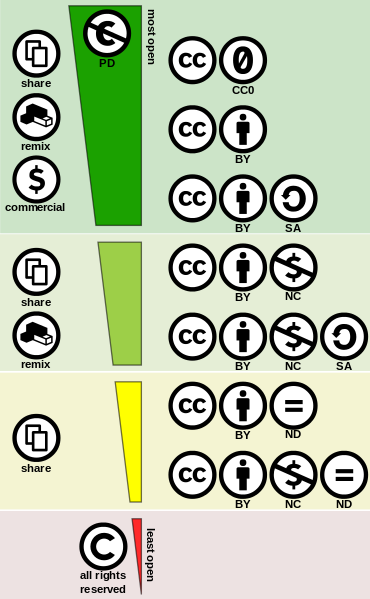
\includegraphics[width=.5\textwidth]{pictures/Creative_commons_license_spectrum}
 \caption[Creative commons license spectrum between public domain and all rights reserved.]{Creative commons license spectrum between public domain (top) and all rights reserved (bottom). Left side indicates the use-cases allowed, right side the license components. The dark green area indicates Free Cultural Works compatible licenses, the two green areas compatibility with the Remix culture. \href{https://commons.wikimedia.org/wiki/File:Creative_commons_license_spectrum.svg}{Image by Shaddim via Wikimedia Commons.}}
 \label{fig:ccspectrum}
\end{figure}

\ac{CC} emerged from those meetings and was established as a non-profit organization to address this mission. The original idea was to create a site where people could upload their works to share. That idea was abandoned, however, in favor of creating a set of licenses (in the case of (CC0 \ccZero), not a license but a dedication and in the case of (Public Domain \ccPublicDomain), a validation) that allow artists and creators to mark their works with the rights that they would like to permit for their works, such as allowing people to remix and reuse with attribution, or for non-commercial use only. These licenses had icons associated with the rights so that it was easy for people to see what rights were associated with a particular work. (See \autoref{fig:ccspectrum}.)

The licenses allowed artists and creators to make choices about the permissions they wish to grant. They could require attribution (BY \ccAttribution), forbid or allow modification (ND \ccNoDerivatives), prevent use for commercial purposes(NC \ccNonCommercial/\ccNonCommercialJP), or insist that any derivative work be shared under the same license --- share-alike (SA \ccShareAlike). These could be combined; for example, Wikipedia uses \ac{CC} (BY-SA \ccbysa) which requires attribution and for the derivatives to be shared with the same license. One of the key innovations of \ac{CC} was its communication of these licenses in multiple modes: icons, human readable ``deeds'' that described the license in an easy-to-understand way, ``lawyer readable deeds'' that are legal contracts rigorously developed through a global network of lawyers, and a machine readable system of metadata in various formats to allow software, services and other systems to understand the licenses.

When I joined \ac{CC} as a board member, we were in the process of trying to get the licenses ``ported'' to local jurisdictions around the world, to create a global network and to try to create an enduring organization to manage this.

\subsubsection{Public Domain and CC0 \ccZero}

My efforts to create a public domain mark illustrates the complexity of trying to build open spaces in a world that is connected but that differs deeply over the appropriate laws and norms.

During my time as CEO of \ac{CC} from April 2008 to March 2011, we launched (CC0 - \ccZero), known as ``the public domain license.'' By then the requirement for attribution was so commonly requested that it had become a default requirement in all of the core \ac{CC} licenses. But, we realized that there were cases where attribution was impossible and where marking the works as free of all obligations and as close to public domain as legally possible made sense. Our legal team, led by Diane Peters, worked to coordinate input from around the world to try to make something that worked as best as possible in every jurisdiction. Getting to a single document was a herculean effort.

We had previously had a Public Domain Dedication (renamed Public Domain Certification in 2005) that marked works as Public Domain. But that was confusing because the notion of ``Public Domain'' existed in the United States but not in all jurisdictions. When we launched (CC0 \ccZero), we also launched the Public Domain Guidelines that, together with (CC0 \ccZero), were a template of norms that communities could adopt in a way that was appropriate for them. It encouraged norms from the attribution (BY \ccAttribution) license such as provenance (link back), citation, etc. but in a way appropriate to their community and their medium and in a non-legally binding way --- policed through norms rather than law.

These guidelines were adopted by organizations such as Europeana, the massive online aggregation of European cultural works. The guidelines were in great part informed by those used in the scientific community for projects such as Polar Commons, one of the first users of (CC0 \ccZero).

In October 2010, we released a tool called Public Domain Mark (\ccPublicDomain) to mark works in the public domain. This was an important complement to the (CC0 \ccZero) dedication which was a tool for asserting, to the extent possible under the law, a waiver of rights for works that were not in the public domain. For example, the copyright on works by Herman Melville have long expired, so those works are in the Public Domain, and could be marked as such by the (Public Domain Mark \ccPublicDomain). But if you posted something tomorrow about Herman Melville, it would automatically be copyrighted. If you wanted instead to release the work as close as legally possible to being in the public domain, you would use the (CC0 \ccZero) dedication\footnote{Some legal jurisdictions do not allow you to completely waive all of your rights. (CC0 \ccZero) is a dedication that waives all right to the extent possible under the law. It is also a waiver of rights, and not a license.}. Europeana was requiring that metadata with licensing information be added to all thumbnails indexed on their site. They were planning on creating a Europe-only public domain mark for their site, but we were able to convince them to instead use our Public Domain Mark which that was usable worldwide. 

It gets yet more complicated. The U. S. Government considers works ``prepared by an officer or employee'' of the federal government to not have protection under domestic U.S. copyright laws and regulations. However, the U.S. Government asserts that its employees hold the copyright to these works in other countries. Most people imagine that U.S. Government works such as \ac{NASA} photos or government studies are in the public domain globally, but they in fact are not. This means that Wikipedia, which uses a (BY-SA \ccbysa) license, could not use, say, an image from \ac{NASA} because non-US people could access the pages.

\marginpar{We were emboldened by the fact that the White House had switched the copyright license for the White House website to a \ac{CC} (BY \ccby) license when President Obama was inaugurated.}I visited the White House, the Public Printers Office, and a number of agencies in the federal government to try to address this issue, arguing that this restriction made no sense and that preventing U.S. Government works from entering the worldwide commons was impinging on the impact of these works and went against the spirit of creating such works. We were emboldened by the fact that the White House had switched the copyright license for the White House website to a \ac{CC} (BY \ccby) license when President Obama was inaugurated.

With the help of Beth Novack, who was Deputy Chief Technology Officer of the US at the time, I tried to come up with a plan whereby each U.S. agency could use something similar to a (CC0 \ccZero) dedication to give up the international rights to their works so that Wikipedia and others could use \ac{NASA} images and other government works freely on the Internet. Eventually, I ended up at the \ac{GSA}, where I was told that federal agencies do not have the right to waive their copyright and that the international rights were ``assets of the federal government.'' Moreover, the \ac{GSA} controls the federal government's balance sheet and thus has to approve any such transactions.

This issue has still not been resolved and is still being actively pursued by \ac{CC}.

\subsubsection{Interoperability}

An issue came up in Europe around a right called a ``database right,'' which provided protection to databases or collections of works even if the individual works in the database weren't copyrighted or able to be copyrighted. The United States and many other jurisdictions didn't have such law or right, and addressing it in the (CC0 \ccZero) dedication or \ac{CC} licenses didn't make sense from a global perspective.

That led the Open Knowledge Foundation, a friendly partner in the United Kingdom that often helped us in the region, to create an Open Database License to deal with the database issue. But this license was not interoperable with and, in some cases, tried to replace \ac{CC} licenses. One key example was OpenStreetMap, an extremely important crowdsourced source of open maps used by many services such as Foursquare and Craigslist. OpenStreetMap originally used (BY-SA \ccbysa) license but the organization was convinced to convert to Open Knowledge's ODbL license. We had many conversations to try to keep them with \ac{CC}. While the ODbL dealt with database rights in a way that \ac{CC} didn't, we believed the benefits of ODbL didn't outweigh its cost, namely, that OpenStreetMap data would no longer be interoperable with other (BY-SA \ccbysa) works, including huge projects like Wikipedia.

Similar to technical protocols such as \ac{TCP/IP}, even if the legal ``code'' of the licenses are nearly identical, they are slightly different and make interoperability difficult, if not impossible. The key thing about share-alike or copy-left licenses is that they require derivative works to be licensed under the same license. So even if the licenses are nearly the same, because they are not the same license, the user can't switch the license. This keeps the works that are spiritually similar in intent, separated legally. One idea that many of us had was to create a section in the license that listed other, but similar licenses that the user could opt to relicense under. However, since licenses could be upgraded or changed, people didn't feel safe creating a list of compatible licenses because there was no assurance that they would continue to remain theoretically aligned.


In Open Source Software licenses and with those from \ac{CC}, we made efforts to find ways to make different licenses interoperable, but this also required a great deal of work and had limited success. The two most notable examples are the Mozilla Public License 2.0 defaulting \ac{GPL} compatibility and (SA \ccShareAlike) 4.0's compatibility mechanism that is used to make it \ac{GPL} compatible. Additionally, after Wikipedia migrated to (BY-SA \ccbysa), OGL-UK-2.0 and several other open government licenses were made explicitly \ac{CC} (BY \ccby) compatible.

One of the most significant relicense efforts was Wikipedia, which was created before \ac{CC} and established using the Free Document License that the Free Software Foundation created for the GNU free software project to allow free sharing of documentation for its software. It was designed for things more like books and so not well suited for the kind of remixing and editing that Wikipedia represented. For example, it required the distribution of the license with the software, rather than just a link to the software because it was designed before the Web. More importantly, it was not interoperable with the ever-growing body of \ac{CC} licensed works on the Internet because although it was a copy-left license\footnote{A copy-left license, like a share-alike license, allows works to be used freely as long as the derivative works are relicensed under the same agreement. This stipulation first popularized in the GPL software license forces free software to increase rather than just be reused and is the one of the core political features of free software.}, it did not allow relicensing under other licenses such as the \ac{CC} share-alike (SA \ccShareAlike) and therefore could not be remixed with \ac{CC} content that should otherwise have been compatible with Wikipedia.

After a great deal of discussion and negotiation with the Free Software Foundation and the Wikipedia community, \ac{CC} came up with a deal that allowed for a brief period a modification in the Free Document License. This modification allowed Wikipedia to convert its content to a \ac{CC} (BY-SA \ccbysa) license, and in 2009, supported by a community vote, we were able to convert Wikipedia from the Free Document License to a \ac{CC} (BY-SA \ccbysa) license, vastly increasing the body of work available under that license.

\subsubsection{Funding and Organization}

Idealistic intentions require realistic infrastructure. And that requires raising money and dealing with organizational issues. Yet even these activities can be approached in ways that represent the values and methods of antidisciplinarianism.

As a board member and before I became the CEO, I was actively involved in fundraising for \ac{CC}. Fundraising for causes that are hard to categorize and may appear to be ``infrastructure'' is quite challenging. Funders typically like to fund programs or ``verticals.'' In addition, there is a natural tendency for special projects to turn into bigger initiatives and spin out for programmatic and personality reasons.

When I became the CEO of \ac{CC}, we had three projects with separate funders and project leaders. One was ccLearn, which was dedicated to the development of Open Educational Resources (OER) and supporting the learning and education community. The William and Flora Hewlett Foundation funded it. We also had Science Commons, a project aimed at building a ``Creative Commons for Science'' that would focus on issues such as patents and materials transfer agreements. We also had a separate office working on \ac{CC}'s international effort and headquartered in Berlin. Lastly, we had created a group called iCommons. ``The aim of iCommons reaches far beyond the infrastructure that \ac{CC} is building. The aim of the iSummit is to bring together a wide range of people in addition the \ac{CC} crowd --- including Wikipedians, Free Software sorts, the Free Culture kids, Access to Knowledge heroes, Open Access advocates, and others --- to 'to inspire and learn from one another and establish closer working relationships around a set of incubator projects'' \cite{iCommons18:online}.

While each of these projects had a strong mission and purpose, I felt that they were fragmenting the organization and impairing its management and community dynamics. One of the largest efforts --- an intervention that I led with the board and staff --- was to consolidate all of these projects into a single \ac{CC} organization. iCommons, which was already a separate legal organization was made more clearly independent. This clarification and consolidation made \ac{CC} a more integrated and international organization.

One of the keys to success of the \ac{CC} organization and its community was the relationship between the central organization and its regional affiliates. The central organization was a dedicated group of exceptional staff with deep technical, legal and domain expertise in fields such as science, arts and publishing. We had relationships in over 70 jurisdictions, which allowed those partners to use our brand and trademark as long as they adhered to the guidelines in the agreements we struck with them. The use of trademark and brand to manage a network of affiliates had been used in the past, but our use of this structure was quite advanced and effective. Unlike businesses, we did not have a financial relationship with the affiliates and the ``currency'' was the brand. The strength of the brand was sufficient to enforce a high level of adherence to obligations.

 \ac{CC} was not the only organization to strictly protect its trademark while allowing content to be free and open; the Mozilla Foundation takes a similar approach. It provides a useful tool for managing commons-based organizations that rely upon an extended community.

\marginpar{One of the hardest problems was how to keep volunteers --- often the majority of the labor --- sufficiently motivated and organized.}As part of our effort to build a global community while respecting the differences in culture and legal environments, we also ran highly effective international meetings where community members could communicate, collaborate and build trust. We had an extremely diverse group of people in our community ranging from federal judges to artists to communist activists. They nonetheless were able to come together to support a common cause. Strong bonds were built. These connections across traditional boundaries have become an extremely important part of the \ac{CC} community. The events were also critical in providing a way for the volunteers to feel actively involved, and for us to have both difficult and delightful conversations --- I do not think that the organization could have survived at its scale without these physical meetings.

The integration effort, the trademark management, the organization of the international conferences, and the organization in general shared some common themes that we learned and continued to develop, sharing best practices with other organizations with similar structures. One of the hardest problems was how to keep volunteers --- often the majority of the labor --- sufficiently motivated and organized. With a core paid staff, there was always a ``difference in class'' issue with the unpaid volunteers. Also, deciding who was allowed to speak on behalf of \ac{CC} and on what topics, was a key issue that needed to be well managed.

The board of directors was originally all US-based and mostly academic. Over the years, we included a broader representation of geographies and fields.

Managing the brand was key. We needed the kid who wore the \ac{CC} t-shirt and marched in the streets against bad politicians to feel like part of the ``tribe'' but to also make it clear when we were negotiating with the UN which individuals in our system were qualified and authorized to speak on our behalf. The public as well as internal management of inclusion and tight control of key roles appears to similar in every successful open project that I've ever participated in and something that can be applied even to university campuses or companies.

I personally feel a need to point out that all of this online activity occurs in a real world that can impose very real costs. I will always remember Bassel Safadi, a tremendously important member of our community and a key person in developing the work of \ac{CC} in the Arab region, as well as building bridges with other regions. Thanks to Bassel and an exceptional group of colleagues in the region, we launched a set of Egyptian \ac{CC} licenses in 2013. This effort took years of work and many difficult meetings requiring us to learn the relationship between the different countries, the culture, the role of law in the region and bridging many fundamental differences with systems. Bassel was later imprisoned and murdered by the Syrian Government.

We don't know if his work for \ac{CC} played a role in his death. But Bassel's absence reminds us that the funding and organizational work are in service to communities of people who have dedicated themselves to making the world better, often against long odds. These communities are the most significant asset that \ac{CC}, and the Media Lab, have developed.

\subsubsection {Continuing the Work}

While some services such as Flickr made \ac{CC} licenses available to users uploading material as a core part of the services they offered, it took years of work to persuade YouTube, Google and many of the large Internet platforms to embrace our licenses.

I remember giving a talk at a publishers conference many years ago where I shared the vision of \ac{CC}, explaining that its licenses helped authors who wished to share their works without making people ask them for permission. When I finished, the first publisher to rise to comment said, ``I think your comments are disgusting.'' She pretty much summed up the feeling in the room. 

We've come a long way. In March 2018, I gave the keynote address at the MIT Library conference on Grand Challenges where I was asked to talk about open scholarship. I noted that even the publisher with the most stringent copyrights, Elsevier, now uses \ac{CC} licenses to mark their Open Access works and that \ac{CC} has become a common default for publishers, authors and others to assign whatever rights they wish to their works. Many foundations now require their grantees to publish their works under \ac{cc} licenses, and the licenses have become a key element of the Open Access movement to free academic works for sharing, and for scientists to use the Internet to its full potential.

\subsection{The Open Source Initiative}
\label{sec:OSI}


\cite{Historyo84:online}:
\begin{quotation}
Development based on the sharing and collaborative improvement of software source code has a history essentially as long as software development itself. In the late 1990s, interest and participation in this phenomenon increased markedly with mainstream recognition of Linux in publications like Forbes and the release of the Netscape browser’s source code.

The \ac{OSI} was formed in 1998 as an educational, advocacy, and stewardship organization at the important moment in the history of collaborative development.
\end{quotation}

Founded in 1998, \ac{OSI} was a campaign to promote open source software. Having created the ``\href{https://opensource.org/osd}{Open Source Definition}'' that became a standard definition for ``open source.'' \ac{OSI} developed a board of directors and became the organization that reviewed and ``approved'' open source licenses tested against the Open Source Definition and granted permission to use the \ac{OSI} mark.

\begin{figure}[h]
 \centering
 
\includegraphics[width=.5\textwidth]{pictures/Opensource}
 \caption{The \ac{OSI} logo}
 \label{fig:OSI}
\end{figure}


The organization also aimed at pushing back against what many believed was an effort by commercial software companies to fight the move toward free and open source software. These fears gained credibility when, in October 1998, confidential documents known as the ``Halloween Documents'' \cite{Hallowee48:online} were leaked to Eric Raymond. They revealed Microsoft's strategy against Linux and Open Source software, confirming the community's fears that Microsoft and others were engaging in an all-out war against Open Source.

I joined the \ac{OSI} board in May 2005 and served for two years and two months. During this period we worked on a number of issues.

One issue was license proliferation. Just as with \ac{CC} licenses, the interoperability of \ac{OSI}'s licenses was crucial, but the number of similar yet incompatible licenses was growing. There were already a number of open source licenses, but during my tenure, we saw a number of ``vanity'' licenses being created: licenses created by companies or communities solely for their own projects and with little consideration for the damage to interoperability. As with \ac{CC} licenses, small changes made software licensed under these modified derivative licenses incompatible with other software licenses, preventing developers from combining code from different projects. Having too many licenses to choose from also made it difficult for developers to choose one. 

We decided to intervene and embarked on a mission to try to talk people out of vanity licenses. We were successful in getting a number of licensees deprecated, including Intel's own Intel Open Source License \cite{LicenseP82:online} ; it was nearly the same as the popular BSD license, but with a clause regarding export laws.

\marginpar{A key learning for me was that with open protocols there is a period where many ideas proliferate and innovation occurs. This is important. However, it is important to work on converging the standards as the network and projects deploy.}Nations are one of the more stubborn ``disciplinary boundaries'' we face as we try to build global communities and communities of practice in a world that is always local. We saw this again with the Mozilla license. (I later served on the Mozilla Foundation board.) It stipulated that disputes must be handled in Santa Clara County, California, but most companies basing their license on the Mozilla license substituted their own jurisdiction, which created a substantial number of incompatible but very similar licenses. This was eventually resolved in \href{https://opensource.org/licenses/MPL-2.0}{version 2} which set the jurisdiction to ``where the defendant maintains its principal place of business.''

A key learning for me was that with open protocols there is a period where many ideas proliferate and innovation occurs. This is important. However, it is important to work on converging the standards as the network and projects deploy. For example, in the cryptocurrency space, we see a proliferation of blockchain technologies, that will hopefully begin to converge soon.

During my \ac{OSI} tenure, the key to the success of \ac{OSI} was the strong leadership of Michael Tiemann and Danese Cooper.I learned a great deal from their management of the organization and the stakeholders.

\subsection{Blockchain and Questioning Sovereignty}

Blockchain has become the IT ``fad du jour'' and is being touted as the solution for almost everything. It is clearly hyped right now, but the ideas behind it have been around for a long time and I believe that the impact will be larger, different and later than most believe. Similar to the Internet, its decentralizing and unbundling architecture will drive a similar, if not equivalent, change in the finance and legal fields as well as in other sectors.

In 1995 I predicted that ``for world economies, like a brand new foreign exchange system using digital cash, or a new stock market based on digital transactions --- those are really great visions that will happen, but they will happen based on a need'' \cite{EccosysI53:online}. The next year, I wrote a book about digital cash \cite{digitalcash} with Takao Nakamura, who left the Bank of Japan to join me at the startup I co-founded, Digital Garage. The book surveyed the digital currency projects at the time and charted a vision for the future of digital currencies and electronic payments.

Then my team at Eccosys and I set up a DigiCash server (199.100.7.5) and established an Ecash Merchant account that allowed us to send and receive Mark Twain Ecash, a gold-backed digital currency issued by the Mark Twain Bank in the US. We sold music and images on the Tomigaya website, but DigiCash did not take off and and went bankrupt in 1998. The excitement around digital cash dwindled, although digital payments and settlements continued.

In 1999, Digital Garage, and Lawson's, the convenience store chain, began working together on the idea of turning convenience stores into payment gateways using the Lawson Loppi terminals in the company's stores. I worked with the Digital Garage team to sell the president of Lawson, Naoki Fujiwara, and his team on the vision and help them think about potential applications. Digital Garage, Lawson, Mitsubishi Corporation and TIS Inc. then created a joint venture called eContext, which would become one of the largest settlements company in Japan. The eContext Asia group is a global network and went public at Hong Kong Stock Exchange in 2013. It is now a 100\% subsidiary of Digital Garage.

\subsubsection{Managing disagreement: Cypherpunks}

My work on digital payments piqued my curiosity about cryptography and the Internet, and I got actively involved in the Cypherpunks community, an informal group of hackers who worked on cryptography, networks, and systems. I was fairly active on the group's mailing list, which was the place where most conversations occurred, and I worked to bridge communications between Japanese researchers, governments, and this community. In 1997, I attended a conference in Amsterdam called ``Hacking in Progress,'' which took place in the middle of a forest. The Cypherpunks had set up a tent, where I was able to connect with many community members from Europe as well as the United States.

Many of the key developers and thinkers from this early period are the leaders of the current cryptocurrency field. Many of the ideas that sound new today were hatched during this early Cypherpunk period.

Establishing a conversation between government regulators and the decidedly anarchical Cypherpunk community was never easy. Here's is an example of my attempt to get feedback on some ideas for a Japanese National Police Agency study group. This is from the notorious Cypherpunks mailing list. Tim May is one of the co-founders of the list.

\begin{verbatim}To: Joichi Ito <jito@eccosys.com>, cypherpunks@cyberpass.net
Subject: Joichi Ito as a Junior Policeman
From: Tim May <tcmay@got.net>
Date: Fri, 1 Aug 1997 23:46:56 -0700
In-Reply-To: <199708020550.OAA04024@eccosys.com>
Sender: owner-cypherpunks@Algebra.COM

At 10:31 PM -0700 8/1/97, Joichi Ito wrote:

>I can't tell you about any of the other stuff that is currently being
>presented
>in the study group, but once the report becomes public, I will try to get
>an English version up on the Net. It should end up being the Japanese
>National Poice Agency's official position on Key Escrow, Certification
>Authorities, and several other issues.

And why are you helping to write a report that will be the "official
position" of the Japanese cops?


>I will be participating in another study group soon to discuss many of
>these issues with the Self Defense Force from the point of view of
>Japanese national security as well as another NPA study group on
>what to do about "crackers"... Anyway, if anyone who can give me some
>insight into these areas will be at HIP, I'd love to chat. ;-)

And why are working for the "Self Defense Force" (the Japanese DOD, for
those not familiar with the terminology).

The JDF is notoriously militaristic. You should reconsider this.

And Cypherpunks should be very careful about "advising" an obviously
co-opted member of the Japanese military and police establishment.

Use crypto to undermine such entities, not support them. Crypto will
unleash anarchy on the world.

>Thanks again.
>
>- Joi
>
>P.S. I am not a "policeman" but an outside board member of these
>study groups. The ministries are under quite a bit of scrutiny these
>days and the study groups tend to be quite frank and balanced.
>The reports don't always dictate the law, but since most politicians
>do not have real staffers, therefore most of the expert study
>is done in the ministries.

You sound like a "junior policeman" to me.

Another person to add to the killfiles.

--TCM

--
From: Tim May <tcmay@got.net>
Subject: Re: Tim Throws a "Leaner" / Re: Tim Speaks the Truth
Date: August 3, 1997 at 22:02:24 PDT
To: cypherpunks@algebra.com
Cc: jito@eccosys.com

At 8:46 PM -0700 8/3/97, Anonymous wrote:
>Joichi Ito wrote:
>>As for Tim's message... I keep worrying (when I am in Japan)
>>that I'm too radical, so it's nice to hear from someone who
>>is really hardcore to put a wimp like me in my place. ;-P
>
Actually, when Tim puts someone in what he considers to be their
place,
it usually involves the purchase of a tombstone.

Actually, the trick is to avoid having the body discovered.
What goes into the 10 h.p TroyBilt Chipper/Shredder comes out
not needing any kind of tombstone at all.

Not that I have ever advocated killing mere folks like Joichi
with whom I disagree strongly. (A new quote: "Killfiles don't
need tombstones.")
\end{verbatim}

While the players have gotten older, the style and the tone of many of the conversations on mailing lists about Bitcoin are very similar. This is one of the difficulties that we have in the community today. The style of these conversations on mailing lists or \ac{IRC} are a combination of very sophisticated technical discussions and sometimes childish or politically insensitive interchanges. Bringing government, academia, and the Cypherpunk-turned-cryptocurrency community together remains a non-trivial exercise that I am still engaged in. It's harder than organizing the Internet community; although the Internet old-timers were a bit hippie-like, they were mostly academic and often government funded. So while, they weren't different from their buttoned down government counterparts, there wasn't nearly the kind of gap that exists in the Cypherpunk-government-industry trifecta.

I visited and met with many of the Cypherpunks in the United States and organized visits for them to speak in Japan. I also helped Shuichiro Hanabusa from NHK produce a special called ``Crypto Wars,'' about the Cypherpunks movement. I had conversations with the Bank of Japan and \ac{NTT} Data, which were conducting a digital cash trial. The Bank of Japan was unhappy about some of my public comments about digital currencies, and Mitsuru Iwamura at the \ac{BOJ}'s Institute for Monetary and Economic Studies even canceled a talk I was invited to give at there. Later, Iwamura-san became my mentor. I also got to know Naoyuki Iwashita, who later became head of the \ac{BOJ} FinTech Center.

% \subsubsection{Electronic Signature Service\dw{Candidate for deletion}}

% Mart Saarepera, a cryptography researcher, began working for me at my incubator, Neoteny, in 2001, trying to develop a mechanism platform for authentication and digital signing, or Electronic Signature Service (ESS), with the following properties:
% \begin{itemize}
% \item Low cost compared to PKI (X.509 and similar) and user-owned hardware devices such as smartcards
% \item Easy usability based on software and web interface
% \item Robustness --- highly reliable platform built from components with low reliability
% \item High availability --- scalable to at least 150M users
% \item Patent protection
% \end{itemize}

% I approached \ac{NTT} Data about investing in the project, and we also presented it to officials in Yokohama and those responsible for Japanese Digital Signature Act.

% My business development staff at Neoteny made considerable efforts to justify the market hypotheses for ESS but were unable to develop a plan that regulators or businesses would agree to. In 2002, we presented the project to Professor Jiro Kokuryo at Keio University, and in the spring of the following year, Professor Kokuryo used the project as a case in his International 
% \ac{MBA} course and created a team project to develop a viable business plan.

% Two patent applications were filed, ``System and method for renewing and extending digitally signed certificates'' \cite{saarepera2004system} and an application named ``Fast Signature.’’ A year later we discovered the application by Eric Hughes (US2002/0184504 A1) describing exactly the same invention few months before us.

% The key technical features of Neoteny ESS were published a series of academic papers \cite{ansper2001improving, buldas2003electronic}.


% \subsubsection{Time Stamping Service \dw{Candidate for deletion}}

% In 2003, \ac{NTT} Data suggested a joint project with Neoteny to develop a time-stamping system that the company could use to replace its existing time-stamping service. At the time, \ac{NTT} Data was using a hash-chain-based time-stamping platform licensed from Surety Inc. 

% \textbf{Motivation and Goals}

% The goal of the project was to develop a next-level, version 2.0 time-stamping system platform with the following properties:
% \begin{itemize}
% \item Robustness --- high reliability platform built from low reliability components
% \item High availability --- scalability to millions of clients
% \item IP protectability as Surety had six patents and numerous other patents existed in the field
% \end{itemize}

% \textbf{Project Summary}

% We engaged in a two-month project beginning in June 2003, after having completed a patent infringement analysis in the prior year. As a result, a new hash-chain-based time-stamping system satisfying the \ac{NTT} Data criteria was proposed. One patent application was created \cite{saarepera2010system} and all the key technical results were published in two academic papers \cite{buldas2004provably, buldas2005universally}.

% But \ac{NTT} Data eventually decided not to invest in the project, so the research was continued as a PhD thesis \cite{villemson2002size} supervised by Ahto Buldas. 

% In 2006, the TSS was commercialized under the name Guardtime AS (www.guardtime.com) and is now a leading industrial block-chain provider.

% While this project was ultimately successful, we ended up spending a lot of time working with and talking to large companies. This is exactly the kind of academic to business collaboration that has become so much easier, but this work in 2003 with the digital signatures and time stamping was my initial attempt to do deep R\&D with academics. My key lessons were that we should have been more tightly integrated into the US venture community and the cypherpunk community. 

% \subsubsection{Electronic Cash and Payment Systems \dw{Candidate for deletion}}

% In late 2001, Ahto Buldas attended an ISO standards meeting on time-stamping in Tokyo. He gave a presentation at Neoteny about the state of the art of digitized cash. Professor Mitsuru Iwamura of Waseda University, together with the chief cryptographer at Hitachi, Rojoichi Sasaki were invited, but only Dr. Sasaki attended. 

% Buldas’s presented work on Estonia, where 97 percent of bank transactions had been digitalized but no cash was digitalized. He described the Estonian digital banking system where Internet banks were widely and efficiently used as payment systems. He explained that the efficiency of the system was due to an inter-bank clearing system that charged only a small transaction fee. 

% The scalability of such a payment system as a whole, Buldas told us, depended on the scalability of two independent systems: the intra-bank transaction system and the interbank clearing system. Intra-bank transaction systems are instantaneous, but the speed of interbank payments depends on the clearing system and the main question was whether the clearing system could scale

% Interbank clearing is technically easily to achieve, but it depends on trust relationships between banks. Since trust between two banks is unpredictable, it was impossible to develop an efficient interbank clearing system. 

% So Buldas concluded that the only way to make electronic payments scalable was to digitize cash, or create electronic money. Our team was authorized to work on electronic payment systems and on digital money.

% \subsubsection{Neoteny Digital Money}

% Dr. Iwamura and Dr. Iwashita, our advisers, urged us not try to tackle the problem of digitizing electronic cash, however.

% Saarepera and the team spent a great deal of time trying to find ways to digitalize alternatives to digital money like bearer bonds. Jay Dvivedi, chief investment officer of Shinsei Bank and a Neoteny adviser, pointed out that this effort might be meaningless in Japan. Then Neoteny commissioned an analysis by Deloite-Tohmatsu, which strongly discouraged the team from working on digitalization of cash alternatives such securities, collateral and valuables belonging to clients and suggested we work towards digitalization of electronic documents in general. 

\subsubsection{Early Exploration on Cryptocurrencies}

Some time before September 2001, Sen Nagata, Neoteny's head of R\&D, approached Saarepera about electronic cash and a payment system similar to what we know as Bitcoin today. Nagata asked a series of feasibility questions about a system that would combine a bank and a payment channel, including whether it was possible to have:
\begin{itemize}
\item A model of a payment transaction between pseudonymous accounts 
\item A unique ledger of transactions with a formal correctness condition (predicate) 
\item A stack machine for transaction processing
\item Distributed control of accounts (multi-signature authentication)
\item Cash transfer authorization
\item Cash emission as a special transaction
\item Proof of work, similar to HashCash that guarantees uniqueness of the ledger
\end{itemize}

All the listed items seemed feasible by our team, except the proof of work. We knew about a proof of work from HashCash \cite{back1997hashcash} as a potentially practical anti-spam measure. Saarepera and Nagata had many discussions and concluded that proof of work would guarantee the uniqueness of a ledger only if there was a single ledger and there is not sufficient computational power anywhere to create another one. If we had more than one ledger, proof of work could not be used as a uniqueness criterion.

\marginpar{This early exploration by Sen Nagata is basically Bitcoin. We could have invented it and deployed it years before the Satoshi Nakamoto white paper.}While the work on digital money helped lead to the creation of eContext inside of Digital Garage and sparked my collaboration with Lawson, we should have pushed harder to try to develop true digital cash. This early exploration by Sen Nagata is basically Bitcoin. We could have invented it and deployed it years before the Satoshi Nakamoto white paper.

We may have been too early, but my lesson learned is to not give up on radical ideas just because people tell you that you can't do it. :-)

\subsubsection{Havenco}
\label{sec:havenco}

As the same time that I was straddling the line between hackers and government, I became interested in the cross-border repercussions of the Internet and the role that cryptography and the Internet would play in trade and contracts. I worked with the United Nations Commission on International Trade Law to come up with rules for arbitration in cyberspace, and in May 1999, I presented a proposal for cyber-arbitration at a meeting of the Inter-Pacific Bar Association. The same year, I also worked with the Japanese Ministry of Trade and Industry on the Japanese response to the first discussion of electronic communications at the World Trade Organization. 

I created demos, sat in many long meetings but we never deployed. Lesson : working with government is slow work.

Working on Havenco was the opposite of working with big government.

\begin{figure}[h]
 \centering
 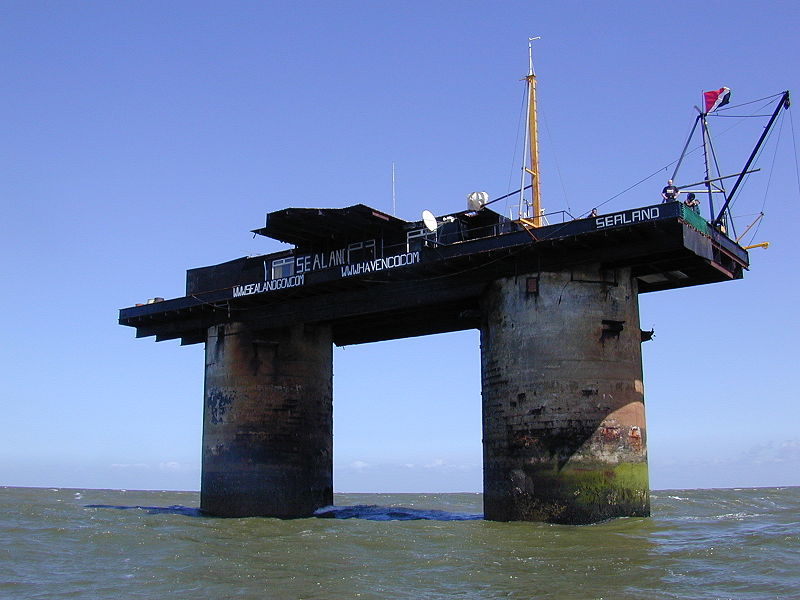
\includegraphics[width=0.5\textwidth]{pictures/sealand}
 \caption{The Principality of Sealand where we ran the Havenco business. Photo by Ryan Lackey.}
 \label{fig:sealand}
\end{figure}

\marginpar{In 2000 it was technically difficult to establish communications with an aircraft platform in the sea. Doing so required a team of engineers and armed guards to live on this old anti-aircraft platform.}In 2000, I took up a quirky project to develop a data center business called Havenco on the Principality of Sealand (see \autoref{fig:sealand}, a tiny nation established on an offshore platform located in the North Sea off the coast of Suffolk, England. We could protect these servers from government spying or seizure --- at least that was the idea. Wired ran the Sealand experiment as a cover story that year \cite{garfinkel2000welcome}.

In the year 2000, Wired Magazine devoted its cover to a story about Havenco \cite{garfinkel2000welcome}. The idea of the company was to take John Perry Barlow's 1996 Declaration of the Independence of Cyberspace \cite{barlow1996declaration} literally and create a co-location/data center in a sovereign jurisdiction that we controlled. 

I met a group of Cypherpunks --- Ryan Lacky, Sean Hastings, Jo Hastings, Avi Freedman and Sameer Parekh --- that were in discussions with the Bates family, who had declared their World War II anti-aircraft platform off of the shore of England a sovereign state: Sealand. They cited salvage law since it was abandoned. At one point, they had fired on the British Navy and were taken to court and their position was upheld.

I became an advisor and an investor and embarked on one of the most interesting but craziest ventures I have ever been involved in.

In 2000 it was technically difficult to establish communications with an aircraft platform in the sea. Doing so required a team of engineers and armed guards to live on this old anti-aircraft platform. (Luckily, I wasn't part of the operations team.) One of the main costs was fuel to power the generators.

The venture was a really interesting idea, but it was early, the team was not experienced enough, and it was a really hard problem. Unfortunately, the project ended before we were able to test some of the more interesting questions in court or on the battlefield.

While it was ultimately unsuccessful, the project was possibly the closest any group has ever gotten to creating a jurisdictionally independent data haven akin to Barlow's vision.

The business plan of Havenco is in \autoref{ch:havenco}.

Through the process of planning and operating the company, we explored in a very real way the challenges and opportunities global communications infrastructures like the Internet face. While inter-jurisdictional challenges were being actively addressed, strange exceptions like Havenco provide an opportunity to imagine other structures. These might come into play again when we start sending servers into space or in the deep sea.

\subsubsection{Bitcoin}
\label{sec:DCI}

In 2008, a person or group of people calling himself or themselves Satoshi Nakamoto (we still don't know who this is) published a paper, ``Bitcoin: A Peer-to-Peer Electronic Cash System'' \cite{nakamoto2008Bitcoin} that kicked off a cryptocurrency mania. The craze started slowly, and I watched it with only mild interest.

But in 2014, Jeremy Rubin, an undergraduate student involved in the MIT Bitcoin Club, nagged me to be the principal investigator on a project aimed at distributing Bitcoin to students to see how they would use it. I was the co-\ac{PI} with Christian Catalini from the Sloan School of Management at MIT. Because of this project, I became more involved in Bitcoin research and supported Jeremy and others who were working in the space. The work was published on their website.

The Bitcoin Foundation became imperiled with an imminent bankruptcy in early 2015. Jeremy and I hatched a rescue plan with support from Adam Back, Pindar Wong, and others in the Bitcoin community. We raised funds and hired key core developers who were supported by the foundation, including the former and present lead maintainer of the Bitcoin project. We created the \ac{DCI} at the MIT Media Lab to house these developers and serve as a nexus for cryptocurrency research.

We have assembled an extremely diverse, relevant and high quality team of experts at the \ac{DCI}, giving preference to those with no commercial interests in any fintech startups or currencies. Directed by Neha Narula under my guidance, the \ac{DCI} has recruited Simon Johnson, the former chief economist of the \ac{IMF}; Robleh Ali, the former head of digital currencies of the Bank of England; Tadge Dryja, the co-founder of the Lightning Network, and Gary Gensler, the former chairman of the Commodity Futures Trading Commission. Our core team is working closely with central banks, regulators and the \ac{IMF}, World Bank, the Inter-American Development Bank (IADB) and others to think and develop long term strategies and protocols that are less concerned about making money and more concerned about creating a working, resilient and decentralized financial system and system of distributed trust. One of the risk of the current focus on for-profit fintech companies is that their focus on financial returns for their founders and investors are driving them to think shorter term and less about a common interoperable infrastructure.

While we still have a long way to go, our work to establish the nonprofit layers of the Blockchain stack is key in trying to make sure that we can create a Blockchain future with fair, functional and interoperable protocol layers, and generative and productive commercial layers in between, following the Internet's model.

The \ac{DCI} has also helped organize the Scaling Bitcoin conference series, which has served as a neutral meeting ground for Bitcoin developers and scientists to discuss the latest research. The first two instances of the event in late 2015 helped diffuse tensions building around the debate over block size, and at the second event, Pieter Wuille, a prominent Bitcoin developer, announced SegWit, or ``segregated witness,'' which offered a way to limit block size; it has become the focus of the technical debate ever since.

Dr. Narula has a background in distributed systems. She and the \ac{DCI} currently are working on the following:

\begin{itemize}
\item Supporting core Bitcoin development
\item Attacking pressing problems to deploy cryptocurrencies in the real world --- for example, how do we provide privacy along with support for insight and financial regulation? How can we create new ways of proving that institutions are complying with financial regulation?
\item Figuring out Layer 2 (not to be confused with layer 2 of the Open Systems Interconnection (OSI) stack) --- blockchains fundamentally don't scale and Ethereum's model of executing every step of every smart contract on chain isn't going to work. We are exploring ways of making payments and smart contracts off-chain, while anchoring trust back onto the blockchain.
\item Redesigning the way that Bitcoin validates transactions to drastically reduce the cost of running a full node 
\item How to take lessons from cryptocurrency and apply them to the problem of designing a digital fiat currency
\end{itemize}

\subsection{The Startup Ecosystem}

My experience as an entrepreneur and a participant in the protocol and non-profit layers of the Internet has been key to my understanding and success at both. 

The Internet startup ecosystem is one of the best examples of the decentralization caused by the diminishing cost of innovation. In \textit{Regional Advantage}, AnnaLee Saxenian describes the shift of innovation from the Boston area to Silicon Valley as innovation in computers shifted from big companies and research labs with lots of money and equipment to smaller startups in Silicon Valley \cite{saxenian1996regional}. This push of innovation to the edges was an extremely important architecture shift that increased generativity in the commercial layers of the Internet. 

In 1999, I set up an incubator called Neoteny, which means the retention of childlike attributes into adulthood. It can refer to all the great things you often lose in adulthood, such as curiosity, playfulness, imagination, joy, humor and wonder. I first learned about the word from Timothy Leary \cite{TheMeani97:online}. I established Neoteny to help startups in Japan develop and as a way for me to develop and support the ecosystem of startups there by applying what I had learned as a startup entrepreneur to . After raising tens of millions of dollars from investors, I rented space and hired forty very smart people to support the startups. I learned the hard way that the cost and management overhead of running a full-service incubator was not commensurate to the value it would add to startups, at least the way I had designed it. The market crashed just after we got started, and publicly traded incubators that were trading at many multiples of the value of their portfolios started trading at a discount to their portfolios. We struggled to morph the model into a consulting company, but I realized that it wasn’t working and eventually let almost everyone go, and returned the remaining money to investors. It was an expensive lesson, but we did some important and original work on cryptography in the R\&D unit that I will describe in the next section. The people who worked at the company, whom I feared I had harmed greatly, developed a strong bond that continues today in the form of collaborations and reunions. Many of the alumni have been very successful in startup ecosystems around the world. 

During this period, I met the now well-known Silicon Valley investor Reid Hoffman. While at Neoteny, I helped him with his strategy to bring PayPal (where he was then an executive vice president) to Japan. I used my relationships at the Bank of Japan to secure a letter explaining how not to be regulated in Japan --- they just needed not to provide any services in Japan. PayPal successfully launched in Japan and Reid and I became friends. I continued investing as an angel investor, learning about the Silicon Valley ecosystem and comparing its robustness with the Japanese startup ecosystem. I realized that the style and network of investors in Silicon Valley, as well as the risk averseness of Japanese entrepreneurs, made a significant difference in the strength of the ecosystem, and I redirected my focus to Silicon Valley. 

After the dot-com bubble burst, sending the prices of technology companies listed on NASDAQ down to pre-Internet levels, Silicon Valley was cleared of irrational exuberance and left with entrepreneurs and investors that truly loved the technology and the work. I invested in a number of companies with Reid, including Flickr and Last.fm, and began developing a network of entrepreneurs and venture capitalists in the region. 

I also began exploring startup ecosystems around the world, including connecting with the community in Singapore, which was more entrepreneurial than Japan. The Singapore government was excited about supporting the ecosystem of startups there. In 2009, I set up venture fund (I currently call it Neoteny 2) with a special provision from the Singapore government that would provide a convertible loan worth 6 times the amount that I would invest in a startup if the startup were domiciled in Singapore. I could buy out the loan at cost, which effectively would provide me with 6 times the upside exposure for the same investment amount — a great deal. Singapore would help me with visas and many other things. I designed the fund so that it was also permitted to invest in non-Singaporean companies. The fund was successful, but ironically through companies that did not use the government incentive.

\marginpar{While some people focused on a particular layer and devoted their life to the development and stewardship of that layers, I expanded the layers that I participated in and used the contact that I had with each layer to try to coordinate and develop a kind of sensibility across the layers.}

From this experience I learned that startups are great for speed, execution and a certain kind of innovation and creativity, but the short-term nature of funding eventually drives companies towards profits and away from many of the societal goals and bigger ideas that may have provided their initial impetus. (This is obviously one reason I was excited to join the Media Lab.) I also found that I personally do not enjoy spending time with most venture capitalists. While they are more thoughtful and less zero-sum than most financial types, the conversations still revolve around money and how to make it. 

I also learned that success in a competitive venture ecosystem is not just being competitive or a hard negotiator, but adding value to the companies and the ecosystem. Great entrepreneurs and companies have their pick of investors; for the best companies, it's a seller's market. Venture capitalists that are successful are generally, although not always, very helpful, smart, friendly, and collaborative. The key to success is to be invited into a round by an entrepreneur or another investor because of what you can contribute to the company --- connections, mentoring, ideas, elbow grease. In successful and vibrant startup ecosystems, a network of investors that will take big bets on big ideas and not push companies to profitability too early is important to establishing ecosystems like Silicon Valley. 

The difficulty is that such an ecosystem requires good entrepreneurs, professional managers and technologists, and a critical mass. It is very difficult to start an ecosystem from scratch, as I learned in Singapore. Boston has an interesting ecosystem, very different from Silicon Valley’s. Boston’s strengths are biotech and the connection to the city's vibrant academic community. During a recent confab in Silicon Valley, nearly all of the leaders said that they ``wouldn't notice'' if Stanford disappeared. No one in the Boston area would say that about Harvard or MIT. The argument was that Silicon Valley attracted talent from around the world, from Stanford and MIT and Harvard, so it didn't matter that Stanford was close by. While the diminishing cost of innovation did push innovation to ``the edges'' and away from big, institutional R\&D centers, it ended up creating a localized ecosystem because of the value of face-to-face interaction and the ability to recruit as companies scaled. Silicon Valley is the clear leader and so is sort of a ``center'' now and not an ``edge.'' 

I believe that biotech has a different formula for developing and commercializing technology and that models such as PureTech Health, which I describe later in this chapter, are possibly more suitable.

% \section{Building a New Public Sphere}
% \label{publicspherepractice}

\subsection{Building Layers of Interoperability}
\label{sec:PSI}

As I participated in building various layers of the Internet, my experience and access to the community of the lower layers, gave me access to, and a starting point for, helping to build the next layers. While some people focused on a particular layer and devoted their life to the development and stewardship of that layers, I expanded the layers that I participated in and used the contact that I had with each layer to try to coordinate and develop a kind of sensibility across the layers.

\begin{figure}[h]
 \centering
 
\includegraphics[width=.5\textwidth]{pictures/Joibathroompop1994.jpg}
 \caption{The PSINet point of presence in my bathroom circa 1994}
 \label{bathroompop}
\end{figure}

One of the benefits of having a 128K leased line to the Internet and the first commercial Internet service provider in Japan in my bathroom in 1993 was that it attracted hackers.

At \ac{ASIJ}, I used to co-run the Computer Club, and Cyrus Shaoul, a former \ac{ASIJ} Computer Club member (much younger than me) and a recent graduate of MIT reached out after he read an article by Howard Rheingold about my Multi User Dungeons (MUD) obsession \cite{kelly1993dragon}. He brought with him several friends including Daishi Harada, another MIT alum, and Sen Nagata and and Jonathan Haggan, both \ac{ASIJ} alumni. They all started hanging out (and sleeping) at my apartment, turning it into a hackers den where we worked on the new Internet software toys as they came out. We did a lot of work with early slowscan TV and CU-SeeMe, WAIS, Gopher, an anonymous remailer, a listserv and eventually the NCSA HTTPd server, which we used to set up our website in 1993.

When we set up our first real website, called ``Tomigaya,'' at \href{https://web.archive.org/web/19961227001638/http://eccosys.com:80/}{eccosys.com} in 1994, it was one of just a handful of websites in Japan. It became the home of many experiments, including an ecash site that sold music and images in exchange for the Digicash ecash that was issued by Mark Twain Bank.

I published a number of books during this period, including a book about cool websites called \begin{CJK}{UTF8}{min}インターネット7日間の旅\end{CJK} [The Internet in 7 Days] \cite{takemuraito} with Mitsuhiro Takemura, a book about how to make your own home page, and in 1996, a book called \begin{CJK}{UTF8}{min}デジタル・キャッシュ―「eコマース」時代の新・貨幣論\end{CJK} [Digital Cash - New Monetary Theory in the Age of E-Commerce] \cite{digitalcash} with Takao Nakamura, following up our experiments with ecash and our study of cryptocurrency at the time.

\subsubsection{Blogging}
\label{sec:blogging}

\begin{figure}[h]
 \centering
 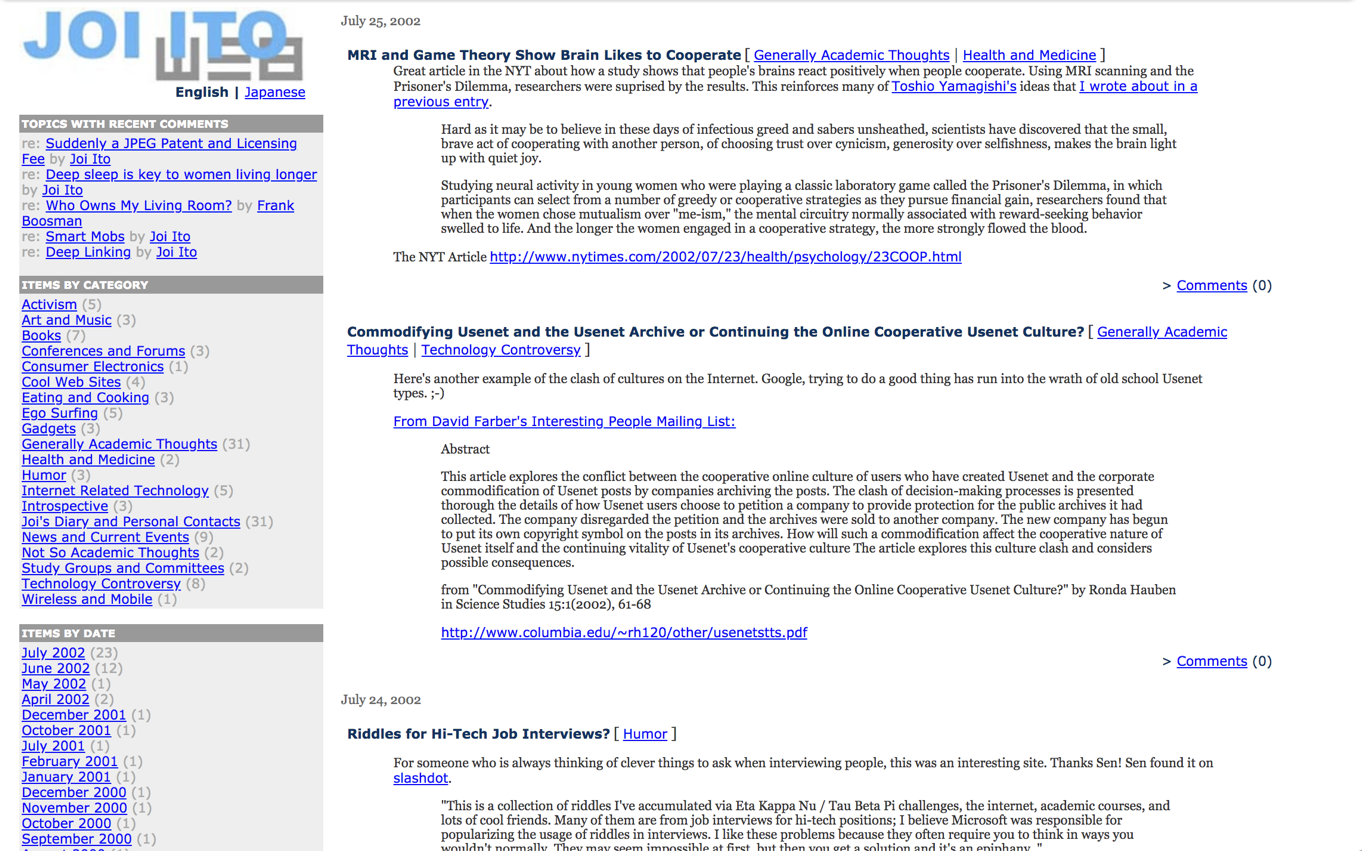
\includegraphics[width=1\textwidth]{pictures/joiblog}
 \caption{My blog in 2002.}
 \label{fig:joiblog}
\end{figure}

In 2002, I converted my personal website, which had a journal section, into a blog (see \autoref{fig:joiblog}) with the help of Justin Hall, who was arguably the first blogger on the Internet; he has been journaling at links.net since 1994. For my site, we used the blog software Movable Type and moved the journal entries from my personal website to the blog.

The big difference between the blog and my journal was that the blogging software made updating the website extremely easy. Posts could be written into a web interface instead of writing \ac{HTML} by hand, which I originally did, or using website design software such as Dreamweaver. Movable Type was open source and allowed plugins, and my team at Neoteny, led by Daiji Hirata, localized Movable Type for the Japanese context. We ended up investing in Movable Type and supporting it in Japan.

The fact that blog software was open source and that there was a community of blog software developers at the time were important factors in the rise of blogging. The community created open protocols like trackbacks, which allow blogs posts to receive the \ac{URL}s of blogs posts that link to them so that the linkbacks can be posted at the bottom of the blog posts. Most blog platforms and systems also allowed users to download all of their content and port it to another blog platform, a feature that was no longer available after the platforms became more commercial or were acquired by large companies.

Interestingly, Japan had had a long history of online journals, or ``nikki'' sites, and the community in Japan on sites such as 2chan attacked us quite vigorously because they believed that bringing blogs to Japan was unnecessary. This included a letter from the chairman of the \begin{CJK}{UTF8}{min}全日本電子日記協会\end{CJK} [All Japan Electronic Journal Association] complaining about the redundancy. I argued that the nikki sites weren't interoperable and that, in contrast, blogs were setting a global standard. I continued to be attacked until some of the standards we developed around blogging took off with the help of some larger companies that adopted them.

\subsubsection{RSS}

One example of a blogging related standard is \ac{RSS}. \ac{RSS} would eventually drive Google Reader and become the core way that many sites syndicated their content.

\ac{RSS} originally started at Netscape and was called \ac{RDF} Site Summary. This was version 0.9. After AOL acquired the company, Netscape dropped \ac{RSS} support from My.Netscape.Com and removed all documentation and tools. The \ac{RSS}-DEV Working Group produced \ac{RSS} 1.0, which reintroduced \ac{RDF} and added XML namespaces and metadata vocabularies -- in other words, making \ac{RSS} more complex and standard. David Winer, a blogger and the developer of the popular blog platform Radioland, then developed a version of \ac{RSS} in 2002 that was substantially simplified and called it \ac{RSS} 2.0, eventually renaming it ``Really Simple Syndication.''

Not surprisingly, this inspired a great deal of dispute and argument, with the \ac{RSS} 1.0 people arguing that \ac{RSS} needed to be extensible, robust and tied into other global standards. Dave and his \ac{RSS} 2.0 supporters argued that \ac{RSS} needed to be easy for developers and users to read and write to and that all of the complexity in \ac{RSS} 1.0 was unnecessary. This was only one of the many standards debates that occurred online at the time, but because of the emergence of blogging as a communications platform, we were able to have these debates on our blogs. 

I invested in and started working with a company called Technorati that aggregated blogs so that they could be searched --- Google was not yet paying attention to blogs -- and the links among them could be tracked. I also invested in a company called Blogrolling that built a tool that allowed bloggers to manage a list of their favorite blogs that would show up on the side of their own blogs. I also invested in a company called ECTO that allowed its clients to post to any blog platform that supported XML-RPC, a standard for programatically posting to blogs.

Through the conversations on my blog, experimenting with these standards myself, meetings that I attended or hosted,and nudging the companies that I invested in, I contributed to moving these standards forward. For example, in 2003, Ben Trott, the developer of Movable Type, and Dave Winer agreed to a standard change in the metaWeblog \ac{API} after a short exchange in the comments on my blog \cite{metaWebl87:online}. The way that we discussed these standards on our blogs became the basis for thinking about the future of online conversations.

\subsubsection{Emergence of Social Media}
\label{sec:emergentdemo}

I have a category on my blog called ``blogging about blogging.'' with over 500 entries. Through this process of arguing, fighting, agreeing, developing and becoming friends, we bloggers realized that a new kind of social network and governance system was emerging. The term ``emergent democracy'' was coined by Ross Mayfield, who was a member of our community. In 2003, I convened an online meeting --- a phone conference call --- where we discussed this phenomenon. The first call included Clay Shirky, Ross Mayfield, Pete Kaminski, Gen Kanai, Liz Lawley, and Sébastien Paquet, an impressive bunch. I wrote a first draft and then received input from the community on the paper in \autoref{emergentdemo} called ``Emergent Democracy'' which became the basis for a book called \emph{Extreme Democracy}. The final version of the paper is version 3.2 and is on my website \cite{1Emergen42:online} and an except is included in this dissertation in \autoref{emergentdemo}.

The paper contends that blogs were the first version of the phenomenon of online conversations that would change the way that democracy works. My hypothesis was that the current system of representative democracy in which we vote for representatives who deliberate and decide on policy on our behalf with the traditional news media reporting back to us is outdated. People can do more than vote: we could discuss and cause collective action directly through a self-organizing principle in the same way that the development of free and open source software had shown that we can collaborate without formal organizations. Clay Shirky calls this ``the power of organizing without organizations.'' The discussion and the paper itself were written in an emergent way, and it kicked off a movement to discuss and deploy means of governing ourselves through online communities.

In 2003, Howard Dean was a candidate in the Democratic primary in the United States, and I was invited to join the Dean campaign's Net Advisory Net, which offered advice about an online strategy for him. Many members of the network of bloggers were involved, and the Net helped pull off what was one of the first Internet driven political campaigns. I was quoted in Wired Magazine \cite{wolf2004internet} at the time, saying, ``You're not a leader, you're a place. You're like a park or a garden. If it's comfortable and cool, people are attracted. Deanspace [the Dean campaign's very early social network] is not really about Dean. It's about us.'' The campaign was really an online community. Even though the campaign was unsuccessful, its use of an online strategy and convening of an online community redefined the way political campaigns are conducted in the United States, as Joe Trippi wrote in a book about the experience, \textit{The Revolution Will Not Be Televised : Democracy, the Internet, and the Overthrow of Everything} \cite{trippi2004revolution}.

In retrospect, the paper ``Emergent Democracy'' was overly optimistic but nonetheless prescient about the fall of mainstream media and movements like the Arab Spring. When we wrote the paper, I believed the system would would figure out how to self-regulate and build another system more stable and better than the one that we had. I did not anticipate the inability of the revolutionaries of the Arab Spring to rebuild their countries or foresee issues such as so-called fake news. I also believed that conversations about democracy and governance would continue on decentralized systems and did not predict the power of platform companies like Facebook to centralize, aggregate and effectively mediate and control these conversations. I have also been surprised by our inability to contain anger, trolling, and hate speech on the Internet. Somehow I had hoped that once everyone was connected, we would all become friends.

I had my first experience with trolls when I set up a mailing list called ``Netsurf.'' I was working with \textit{Wired Japan} on its version of the Net Surf page of \textit{Wired} in the United States, which had Net Surf page from 1993 that listed interesting \ac{FTP} sites, Usenet newsgroups and email addresses. My Eccosys team set up a mailing list in February of 1995 to share links and talk about the Wired page. We ran the mailing list on our Sun SPARC 1+ and anyone in could join.

Although Netsurf began as a place to share new websites, it evolved into a virtual community where people came to talk about all kinds of topics online. At one point, a member began behaving in what I believed was an anti-social way, and so I told him that he needed to behave more respectfully and civilly. Since the mailing list was on my server and was the space was my virtual living room, I thought that members should follow my rules. But the members argued that the mailing list was a public space, and they didn't care what I said. I learned another lesson --- just because I ran the platform didn't mean I could control the conversation or the community.

As an aside, this was at the same time that ``Jerry and David's Guide to the World Wide Web,'' which turned into Yahoo! in 1994, was starting up, the Eccosys team was talking to Jerry Yang and David Filo about collaboration. We had agreed to do Yahoo! Japan with them, and the first time I met Jerry, he was asleep under a desk at Stanford University where they were getting started. Unfortunately, after I mentioned how exciting Yahoo! was in a conversation with Masayoshi Son of Softbank, he invested in Yahoo! and gained the rights for Yahoo! Japan for Softbank as part of the deal. Son-san asked us to set up Yahoo! Japan for Softbank, and I asked for fifty percent of the Yahoo! Japan business, which I thought was fair since we had originally thought we would have all of it before that. He agreed to give us about one percent of Yahoo! Japan. I told him that I'd rather be paid in cash, and we set up the beta version of Yahoo! Japan for him. Of course, I should have settled for the one percent he offered --- or maybe just kept my mouth shut instead of extolling the virtues of the company to him. But I learned a powerful lesson: investment and financial strength can sometimes outweigh relationships and technical ability.

When our discussions about emergent democracy began developing in earnest, we decided that we needed a real-time chat room to have a continuous conversation. I decided to set up an \ac{IRC} channel because it was open source and very accessible.

Remembering my failure to control my mailing list, I decided to call the channel \#joiito to make it very clear that it was my living room and not a public space. It became a hangout for hundreds of people interested in talking about emerging blogs and social software. Many influential developers hung out in the channel, and many software platforms were conceived and relationships forged there. Stewart Butterfield, who would go on to create Slack, was an active member of our community; Slack is based on \ac{IRC} and his experiences there.

Of course, there was the day that someone came to the channel and asked, ``So what does joiito think?'' After I answered, the person said, ``not you, the channel - \#joiito,'' and then I realized that I had just created another public space. It was called \#joiito.

\subsubsection{Online Communities and Online Learning}

The issue of civility and managing online communities has been one of my core interests and fields of experimentation. My interest in online communities dates back to my first experiences with bulletin board systems in the early 1980s and later services, such as NiftyServe, The MetaNet, Delphi, The WELL, The Source and CompuServe, where the message boards and conference areas were vibrant in content and relationships. In junior high and high school, these systems allowed me to interact with adults and learn through conversations rather than through struggling with textbooks. On The Source, I set up a conference area for every course I was taking in my senior year of high school and talked about the coursework with my friends online. This helped me understand the context of the topics and become more interested in them.

In my senior year of high school, I participated in a monthly meeting of what was called the RINGO Club, an Apple II users group of mostly Americans in Tokyo. I demoed to the group some of the online services I was using. I later started running a regular meeting called TNet, a gathering of the mostly English speaking local BBS and networking community. We shared tips about things like how to rewire the new Epson 300 baud modem to switch between Bell and CCITT so it would operate with US modems and tricks on how to get online. 

At a RINGO Club meeting, I met David Fisher, a retired U.S. Air Force pilot and English language teacher. at the International Education Center in Tokyo and its English language school, Nichibei Kaiwa Gakuin. He had a student named Toshiaki Tanaka, who was the president of a shrimp wholesaler and seafood retailer called Sakako Co., Ltd. Jeffrey Shapard, another English teacher at Nichibei Kaiwa Gakuin, was assigned to do research on educational technology together with Fisher. David connected Jeffrey with Mr. Tanaka and a programmer Tanaka had hired, Makoto Ezure, and they He put together a few entrepreneurial folks who came up with the idea for TWICS, an online communication system. TWICS, which stood for "Two Way Information and Communication System,” launched in 1984 as a system hacked to pick up a phone and connect it to a modem using two acoustic couplers and two Fujitsu personal computers because connecting modems directly to phone lines was still illegal in Japan.
% * <david@weinberger.org> 2018-07-05T19:53:08.975Z:
% 
% >  at the International Education Center in Tokyo and its English language school, Nichibei Kaiwa Gakuin. He had a student named Toshiaki Tanaka, who was the president of a shrimp wholesaler and seafood retailer called Sakako Co., Ltd. Jeffrey Shapard, another English teacher at Nichibei Kaiwa Gakuin, was assigned to do research on educational technology together with Fisher. David connected Jeffrey with Mr. Tanaka and a programmer Tanaka had hired, Makoto Ezure, and they 
% delete
% 
% ^.


When I came home after my first year in college, I spent the summer working on TWICS. We were trying to develop the service beyond a simple BBS. I became an advisor and a member of the TWICS team. 

By 1985, it became a multi-user system and was moved over to a MicroVAX. I pushed to get out of writing our own software and instead license existing software. We started running PARTI, which was the same conferencing system as The Source. TWICS became one of the first public services on X.25 and in 1990 joined JUNet as twics.co.jp. TWICS eventually became an important hub for experimenting with online communities in Japan.
% * <david@weinberger.org> 2018-07-05T19:55:32.949Z:
% 
% > TWICS became one of the first public services on X.25 and in 1990 joined JUNet as twics.co.jp. 
% delete?
% 
% ^.

I also met a number of researchers online who were experimenting with a service called the Electronic Information Exchange System (EIES). It was a multi-user online bulletin board system designed to deliver educational courses and provide a platform for research and communications. It was developed at the New Jersey Institute of Technology (NJIT), and I connected with some of the people doing the early work on it, including Murray Turoff.

In the fall of 1985, The New School offered the first set of fully online graduate courses for credit, and I took two courses, ``Artificial Intelligence \& Life'' and ``Propaganda: Lit Science.'' The propaganda course was taught by a former CIA officer, and the online conversations and content were fantastic --- I remember some of the lessons even today. What's notable about this, though, is that it was happening a decade before the Web and was a very sophisticated use of peer-learning and communities decades before people started talking about Massive Open Online Courses (MOOCs).

Lessons from my activities in communities like this class became the basis of my interest in and my theory of the role of community moderators, peer-learning and the importance of the structure for comments and threads for online discourse.

\subsubsection{Consolidation and Commercialization}

In 1995, Eccosys, my colleagues, Cyrus Shaoul, Sen Nagata, Jonathan Haggan, Hidetoshi Shimokawa, Daishi Harada, Yuki Nakayama and I set up a company for our Internet consulting business. We joined forces with an advertising agency subcontractor called From Garage, which was run by Kaoru Hayashi. We realized that although we dreamed of digital cash taking over the world, all of our income was coming through wire transfers of fiat currency from technology companies trying to promote their Internet products such as Novell Networks, Sun, IBM and others in Japan. At the time, my business skills were minimal and working together with a company that had been in business for more than a decade and knew how to sell services seemed like a good idea.

We worked with the \ac{WIDE} Project for the first time in 1995 on the World Jr. Summit funded by Isao Okawa of CSK. It aimed at connecting children from 40 countries via the Internet. We helped with the technology. That was when I first met Nicholas Negroponte from the MIT Media Lab, who was also working on the project.

That same year, we also built the first Internet cafe in Shibuya, which was sponsored by IBM to promote its new Internet native operating system, OS/2 Warp. The cafe was often the first place that young people without any technical know-how were able to experience the Internet first hand.

Jun Murai and I worked with Carl Malamud to plan and deploy the Internet World Expo in 1996. This was a large project that aimed to connect 80 countries and create online as well as real world pavilions to show people the Internet. Murai-san, the telecommunications companies and the \ac{WIDE} Project worked mostly on the infrastructure, and I focused on content and finding locations, like persuading Mori Buildings to help me create an Internet cafe in Laforet Harajuku.

After losing my shot to run Yahoo! Japan because of Softbank, I was contacted by Infoseek, a automated search engine portal in the United States that wanted my help localizing and launching Infoseek in Japan.

Yahoo!, Infoseek and others had realized  that as personal web pages proliferated, just reading the Netsurf column in \textit{Wired} wasn't enough to keep up with all of the interesting things going on. Even Yahoo! began to have a hard time keeping track of new websites. We realized that a search engine that crawled the Internet, traversing links and finding new websites to create an automatic directory was possibly a key innovation. The theory of ``the portal'' as a consolidated place that would monopolize attention began to take shape.

In 1996, two years before Google was founded, we were using OMRON's SuperMorph-J to do the first ``word breaking''\footnote{Japanese language doesn't use spaces and there is no obviously way to figure out the beginning of a word and the end of a word. This is confounding to search engines. For instance, the name \begin{CJK}{UTF8}{min}山本\end{CJK} [Yamamoto] is two characters, \begin{CJK}{UTF8}{min}山\end{CJK} which means ``mountain'' and \begin{CJK}{UTF8}{min}本\end{CJK} [moto] which means ``root.'' When you search for \begin{CJK}{UTF8}{min}山本\end{CJK} [Yamamoto] you want to find all of the \begin{CJK}{UTF8}{min}山本\end{CJK} [Yamamoto], not every article on mountains along with all of the results for root. A word breaker parses a Japanese sentence, figures out where the word breaks are, and indexes and searches for words rather than characters.} to increase the quality of search.

 Many portals like Yahoo! and Infoseek in the United States had begun to believe that search wasn't as important as offering an array of services such as email, chat, sports and .news. They began to deemphasize search. 

In Japan, Yahoo! and other websites sold advertising in the same way that magazines sold advertising, by a sponsor for a section for a period of time. They would measure how many people saw the advertising, but the advertiser for any page was always the same at any given time. In the United States, Infoseek and others had begun ``rotating'' advertisements and selling advertising by the number of views.

Japanese advertisers and advertising agencies were very much against this method. They didn't like the idea that their advertising might be sharing a page with a competitor. They also didn't like the new way of measuring and selling advertising. Since the advertising agencies were so opposed, we worked with the Kokokunushi Kyokai, the trade group representing advertisers, to run a series of studies and working groups to experiment with --- and get advertisers comfortable --- with the idea of rotating banner ads.

After winning over the advertisers, we worked with a consortium --- Hakuhodo, Asatsu, Yomiko, I\&S and Tokuma Shoten --- to create an ad representation company called the Digital Advertising Consortium (DAC) to initially sell advertising on Infoseek and other websites using this method.

This was the beginning of commercialization of the Internet; the beginning of the advertising driven model for content in Japan, and also the creation of the first ``platforms'' or ``portals.'' Google and search would eventually win over the curated ``network of services'' portals, and simple ad rotations purchased on websites would become a small business compared to adwords and programmatic ad buying.

Blogs would emerge, fueled in part by the search engines pushing traffic to the edges of the Internet. We had long debates about ``the long tail,'' the argument that the lower cost of publishing and distribution would mean only minimal traffic would be needed to support very minor websites. Clay Shirky disagreed, insisting that a power law meant the top sites would become more dominant.

In many ways, he was right, and the decentralized blogging of my youth gave way to the emergence of social media, which changed the architecture from search engines and blogs to centralized platforms.

\subsubsection{Twitter}

In the early days of blogging, Blogger, a blog software platform, was major player in the market. I had been talking to Ev Williams, its CEO, and was trying to develop a relationship with him. I had just offered to invest in Blogger and sent him a term sheet when I learned that the company had been acquired by Google. But I kept in touch with Williams and the rest of the Blogger team, and we remained friends.

Blogger didn't flourish inside of Google and slowly the team left. Williams started working on new ideas, including audio blogs with Noah Glass in a company called Odeo. I was interested in this space, having worked with Nokia and others on multimedia, including being early in setting up mobile blogging or Moblogs. Boris Anthony, who did the design and user interface work on my blog, and Adrian Tijsseling, the creator of Ecto, a system that allowed you to post to blogs from a client, worked together to make make many of the early tools for mobile blogging. At Odeo, they started working on Twitter as an idea for mobile blogging using SMS.

I was intrigued and became an early user. Twitter was clever and created an \ac{API} to allow developers to connect to Twitter, and even though Twitter didn't support Japanese well, many Japanese developers created tools for Twitter. I reached out to Williams and together with Kazuya Minami and Hiroki Eda of Digital Garage, we localized and launched Twitter in Japan. This was early days for Twitter and because Digital Garage had experience selling advertising, we were able to launch a version of Twitter in Japan with advertising even though Twitter in the United States had no advertising at the time.

Digital Garage invested in Twitter and incubated the Japan operations in our offices through a partnership in 2008. Twitter was exciting for me because it was a social hub that sent traffic to blogs and other websites, so it seemed like an interesting and social alternative to search engines. Initially, Twitter appeared to be a great place to have casual conversations about your day and share links with your friends. We didn't realize that Twitter would become the conversation itself, or that the short form of a Tweet, just 140 characters, was more suitable and convenient for people to post content than the longer format of blogs. Twitter also would eventually capture most of the traffic from blog comments, which had been an important part of a blog community. 

\subsubsection{}{Helping Main Stream Media}

The assault on the main stream media that I helped fuel through fighting on the blogger's side of the battle between the amateur press and the professional press was unexpectedly successful. This was only partly due to the quality of the citizen journalism and probably more as a result of the deteriorating business model of mainstream media. Craig's List and other web-based businesses destroyed first the classified ads as a major revenue source. The Internet platforms and online advertising continue to grind away at ad revenues. And while people laughed at Media Lab founder Nicholas Negroponte when he, in the 1990s, suggested that we would be reading news over the Internet, print advertising continues to decline.

As I began to see the demise of main stream media, I joined the board of trustees of the John S. and James L. Knight Foundation in 2011. The Knight Foundation, started by the Knight brothers who ran a US nationwide network of newspapers, created the foundation to engage and inform communities. The foundation focuses a great deal of its efforts in supporting journalism. Through the board, I have contributed to the foundation's support of new business models, understanding the role of social media and investigating the impact of \ac{AI} in the future of the public sphere.

In 2012, I joined the board directors of the \textit{New York Times} and continue to participate actively in the board. The New York Times is one of the few newspapers that has successfully made a transition to a sustainable online subscription model and is constantly exploring new business models and forms of journalism. Through my participation on the board, I have learned a great deal about the business of professional journalism as well as contributed my experience in building and participating in online communities and the creation of content online.

\subsubsection{The Media Lab and the Public Sphere}

Since joining the Media Lab, I have been involved in its Center for Civic Media. The center is run by Ethan Zuckerman, who has been working to understand the public sphere in the digital age and how to interact with it. Media Cloud, a project his group developed together with the Berkman Klein Center for the Internet \& Society at Harvard University, is an excellent example of a tool that can examine how conversations on blogs and media online occur. It lets researchers track ideas and phrases as they move through the mainstream and blog-based channels of the Internet. By looking at such patterns online, Zuckerman and his colleagues can see how communities and news interact to shape the way issues develop in the media.

In their study, ``Breitbart-led right-wing media ecosystem altered broader media agenda'' \cite{benkler2017study}, Zuckerman and his colleagues used Media Cloud to study over 1.25 million stories published online between April 1, 2015, and Election Day. They analyzed ``hyperlinking patterns, social media sharing patterns on Facebook and Twitter, and topic and language patterns'' published by 25,000 sources. ``When we map media sources this way, we see that Breitbart became the center of a distinct right-wing media ecosystem, surrounded by Fox News, the Daily Caller, the Gateway Pundit, the Washington Examiner, Infowars, Conservative Treehouse, and Truthfeed.'' See \autoref{fig:twittermediacloud}.

\begin{figure}[h]
 \centering
 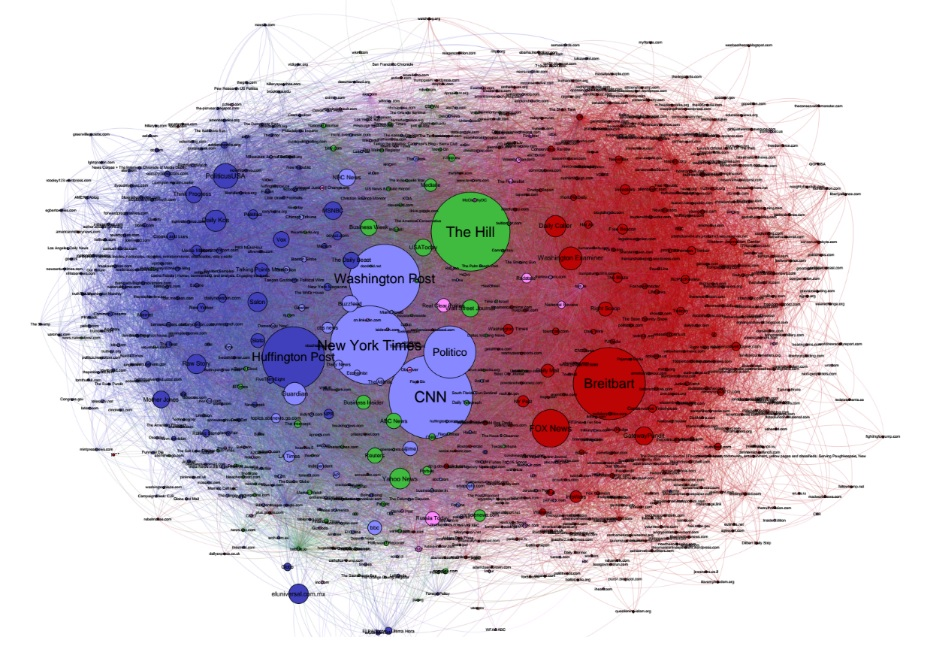
\includegraphics[width=1\textwidth]{pictures/Twitter-Image-1}
 \caption[Media sources shared on Twitter during the election]{Media sources shared on Twitter during the election. (Nodes sized in proportion to Twitter shares. Source: Center for Civic Media at the Media Lab.)}
 \label{fig:twittermediacloud}
\end{figure}

Another group at the Media Lab, the Laboratory for Social Machines run by Deb Roy, deployed the the Electome project \cite{Enterthe97:online} in the 2016 election to look at how supporters of various candidates were connected to each other on Twitter and what they were talking about \cite{electome:online}. Their research revealed how polarized and disconnected these communities were. By mapping the ``tribal networks'' of Twitter users during the elections, as well as some 30,000 journalists on Twitter. they found that almost none of the journalists were in the ``Trump tribe.'' (See \autoref{fig:electome})

\begin{figure}[h]
 \centering
 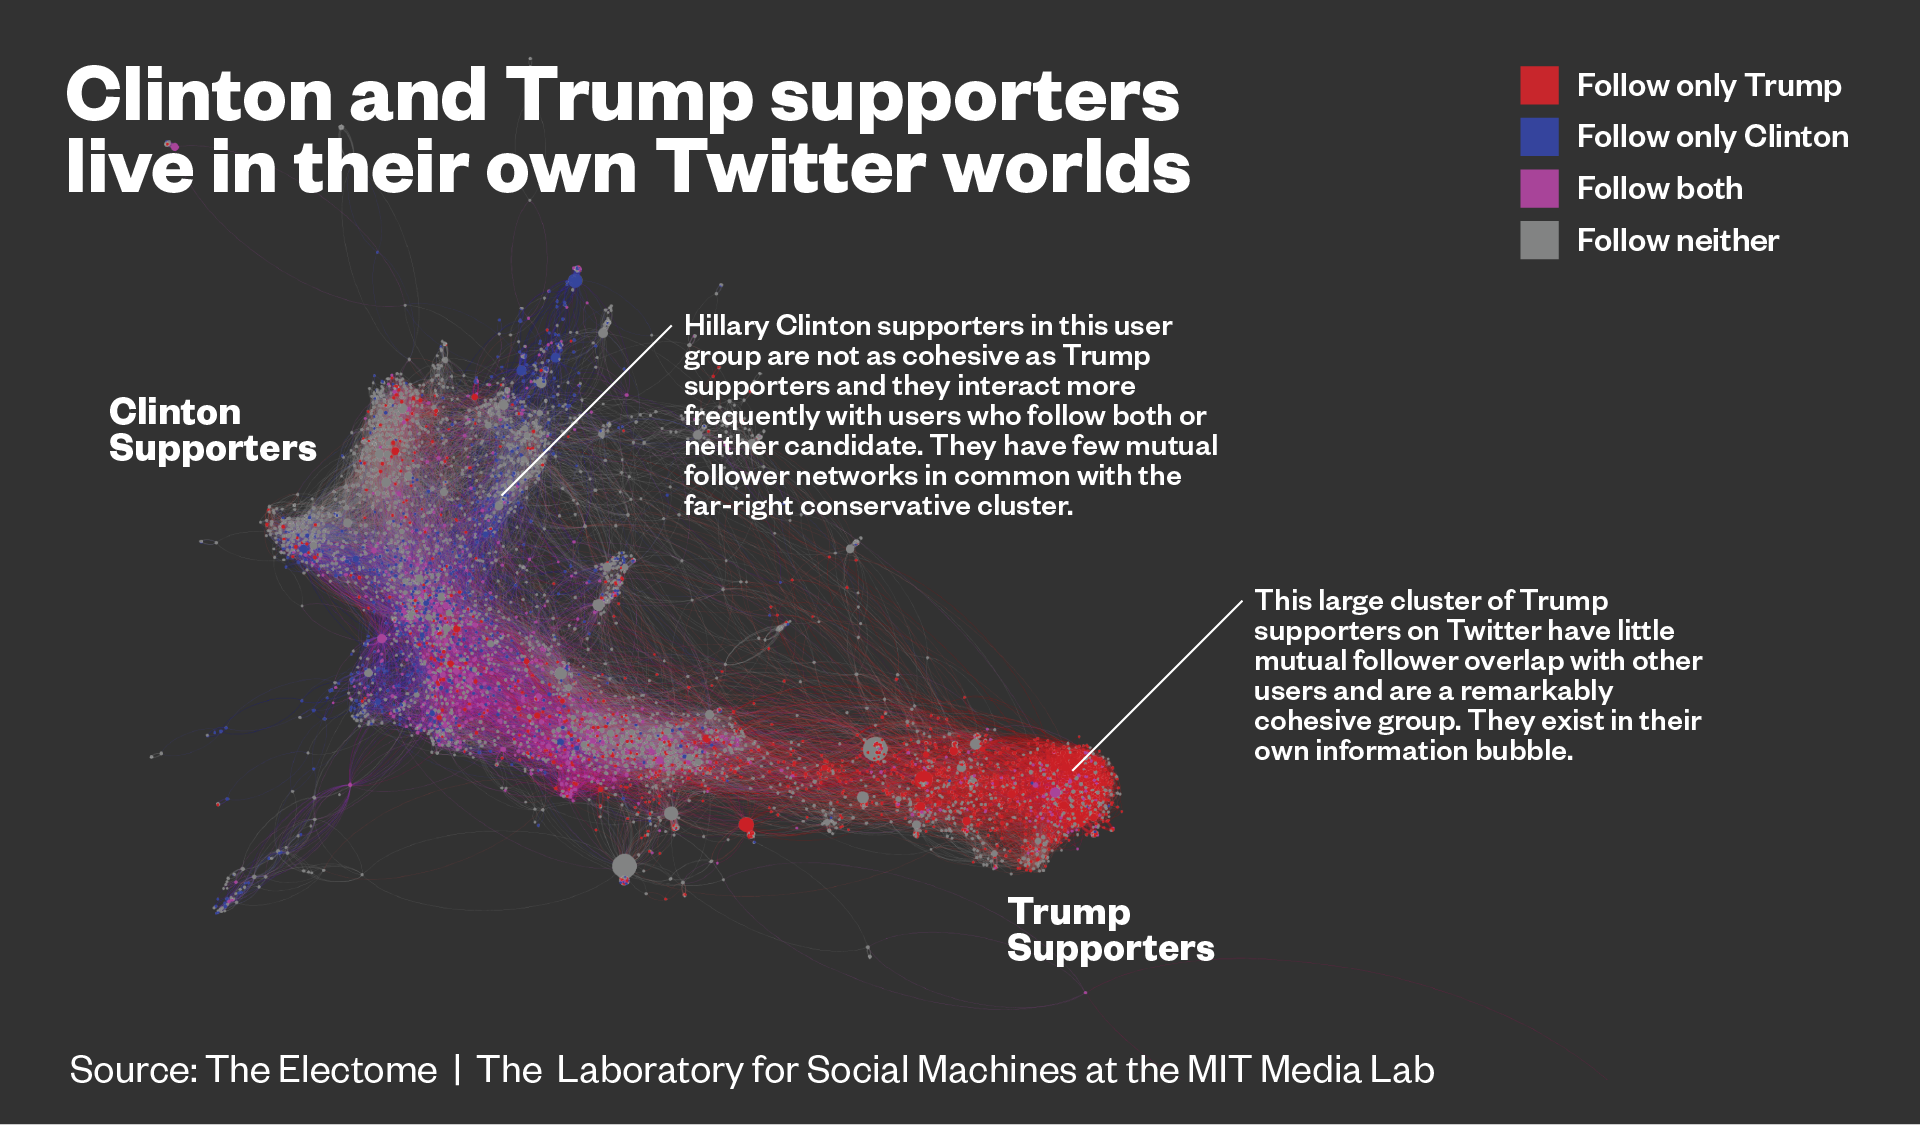
\includegraphics[width=1\textwidth]{pictures/TwitterData1-01}
 \caption[Clinton and Trump supporters live in their own Twitter worlds]{Clinton and Trump supporters live in their own Twitter worlds. Source: The Electome - The Laboratory for Social Machines at the MIT Media Lab.}
 \label{fig:electome}
\end{figure}

In another project, Roy's group has analyzed 11 years of Twitter data to examine the dissemination of rumors as defined by a number of fact-checking sites . The research showed that false rumors spread differently and more quickly  than true stories  do\cite{vosoughi2018spread}. They are also able to show the shape and relationships of the networks of people discussing any issue online. When they analyzed replies to tweets about stories to figure out the emotional response to those stories, they found that ``surprise'' and ``disgust'' were far more often expressed in response to false stories than true stories. This suggests (but does not prove) that in-the-moment emotional response may be a causal factor in why people share stories that turned out to be false. (It also is easier to write a surprising story if it doesn't have to be true.)

Roy's group has  begun to measure shared reality and the civility of the conversations online across different ``tribes'.'  They are also developing public sphere health metrics in a non-profit spin-out from the Lab called Cortico \cite{Cortico96:online}. Cortico is  building tools for local journalists and community organizations to help rebuild community communication, especially in news deserts.

\section{Technology for Social Justice}

\subsection{Artificial Intelligence}

\subsubsection{Ethics and Governance in Artificial Intelligence}
\label{sec:EGAI}

\textbf{Regulatory systems for \ac{AI}}

\marginpar{Our challenge today --- right now --- is to come up with methods to design, audit, and manage the development and the deployment of these systems so that they are socially beneficial.}Watching artificial intelligence and machine learning being developed and deployed so rapidly brings back feelings of watching (and participating in) the Internet in the early 1990s. AI could have an even bigger effect on society than the Internet. But, unlike the Internet it does not appear to be unbundling, or layering, itself. This is a significant issue because while the Internet by its nature was open to users, and derived its value from what users added to it, most AI system are being designed by computer scientists. These systems' effectiveness and bias are determined by the data chosen by computer scientists, and the training and optimization decisions made by them.

Because machine learning systems are trained by providing them with existing data, and because that data almost inevitably reflects existing human biases,  these systems often reinforce those underlying biases. In addition, it is to use the output of AI in inappropriate ways.

Our challenge today --- right now --- is to come up with methods to design, audit, and manage the development and the deployment of these systems so that they are socially beneficial.

I have been engaged in a number of efforts to try to support the introduction of ethics and governance in the development of \ac{AI}.

\textbf{Course on the Ethics and Governance of \ac{AI}}

Harvard Law Professor Jonathan Zittrain and I teach a course on the Ethics and Governance of \ac{AI} \cite{TheEthic48:online}. The course brings students from MIT and Harvard together from disciplines including law, engineering, philosophy, policy, history, and others. The course engages the class in readings, projects and a dialogue around the issues raised by \ac{AI}, as well as thinking about possible solutions.

The key motivation for the course is to try to teach social scientists about engineering, and \ac{AI} and the engineers about the social sciences and \ac{AI}. The course description is:

\textit{This course will pursue a cross-disciplinary investigation of the implications of emerging technologies, with an emphasis on the development and deployment of artificial intelligence. We will cover a variety of issues, including the complex interaction between governance organizations and sovereign states, the proliferation of algorithmic decision making, autonomous systems, machine learning and explanation, the search for balance between regulation and innovation, and the effects of \ac{AI} on the dissemination of information, along with questions related to individual rights, discrimination, and architectures of control. The course will entail an intense array of learning and teaching methods. Students will be expected to participate in a variety of activities. The class may include Media Lab and Berkman Klein Center fellows and affiliates.}

So far, we have been quite successful. A number of engineering students have gone on to become fellows at the Berkman Klein Center and even been admitted to the Harvard Law School. My hypothesis for now is that it's easier to get engineering students interested in a law degree than law students interested in an engineering degree. In any case, the creation of people proficient in both law and engineering is essential for bridging the gap and creating truly creative solutions. However, its likely that we might need a new joint degree program since getting a three-year Juris Doctor (JD) in Law after a degree in engineering seems excessive if the student doesn't actually want to become a lawyer.

The student surveys have made clear the difficultly of having a cross-disciplinary class. Because the class includes law students, philosophy students, computer science students and others, the class has to be accessible to people from other disciplines and necessarily feels shallow to some of them. We should probably experiment with different structures, such as having breakouts to go deep, or to do primers for novices. Another idea would be to have smaller out-of-class dinners or extended office hours to allow some students to go deeper.

Running a cross-disciplinary class in a new area will continue to be a challenge. I hope  we can improve and learn from others.

Together with the course, we have run a program called the \href{https://cyber.harvard.edu/research/assembly}{Assembly}, which brings professionals from industry, academia, government and other sectors to work in teams on  real projects involved \ac{AI}. These ``assemblers'' also participate in the class.

\textbf{The Ethics and Governance of \ac{AI} Fund}

Together with Reid Hoffman, Jonathan Zittrain and Alberto Ibarguen, we have raised a \$26 million fund to support research on the ethics and governance of artificial intelligence. The projects are at the Media Lab, the Berkman Klein Center (where I  have an appointment), and other third-party institutions.

One key design is for teams to work together on projects in an integrated way. The MIT Media Lab and the Berkman Klein Center are the anchor institutions where the largest portion of the funding is directed. We are also directing funding to other organizations that will work closely with us on our key themes. 

We are  uniquely focused on theory and deployment in the real world. The project's work is in three main areas:

\begin{enumerate}
\item Kinetic autonomy --- autonomous vehicles and weapons.
\item Algorithmic justice --- the use of algorithms in social systems such as criminal justice, housing, and insurance, with a focus on bias and the  positive uses of algorithms to improve society.
\item Information veracity --- with the emergence of platforms fueled by targeted advertising and content optimization, we have seen a deterioration of the quality of information and an increase in the influence by outside governments and businesses. What are the problems and solutions?
\end{enumerate}

I am personally deeply involved in the Humanizing \ac{AI} in Law project, which is supported by the fund. We are working to understand the risks of using algorithms in criminal justice, such as using them to generate risk assessments for pre-trial bail. I am also working to use algorithms to understand underlying causal relationships and address systemic problems, rather than just improving the predictive accuracy of algorithms.

\subsubsection{Humanizing Law in \ac{AI} (HAL)}
\label{sec:HAL}

Together with my group, Chelsea Barabas, Karthik Dinakar and Madars Virza, I am engaged in a number of activities including the publication of papers such as ``Interventions over Predictions'' for \textit{Fairness, Accountability and Transparency conference} in \cite{barabas_interventions_nodate} and two letters to the Massachusetts Legislature on pre-trial risk in \autoref{appendix:A} and \autoref{appendix:B}. More recently, I have written the following article for \emph{Wired} about the topic \cite{ItoWiredAI}, and I am speaking a great deal about this.

\textbf{The Church of Prediction and Solutionism}

\begin{quote}
\textbf{When it comes to \ac{AI}, we don't need crystal balls. We need mirrors.}\footnote{Draft of a more academic version of an article written for \emph{Wired}. The final version is available online \cite{ItoWiredAI}.}
 
Critics of artificial intelligence have pointed out the myriad ways that bias distorts the categorizations and predictions generated by algorithms. In response to these concerns, many computer scientists have tried to sanitize their predictive models by identifying and removing ``proxies'' for sensitive social categories like race, in an effort to curb the discriminatory effects of their tools. 

But this colorblind approach to fairness has some serious pitfalls, especially when it comes to addressing the needs of our society's most marginalized populations. For these groups, the core issue surrounding \ac{AI}-enabled decision making is not so much one of accurate prediction and bias, but rather, one of self-determination and social inclusion.
 
This is a topic that my colleague Chelsea Barabas discussed at length at the recent conference on Fairness, Accountability, and Transparency, where she presented our paper, ``Interventions Over Predictions: Reframing the Ethical Debate for Actuarial Risk Assessment.'' (See \autoref{appendix:C} for the full text of the paper.) In that paper, we argue that the technical community has been evaluating the ethical stakes of \ac{AI}-enabled technologies with the wrong measuring stick. By narrowly framing the risks and benefits of artificial intelligence in terms of bias and accuracy, we've overlooked more fundamental questions about how the introduction of automation, profiling software and predictive models connect to socially desirable outcomes.
 
This is perhaps most clearly illustrated in the realm of criminal justice reform, where a variety of predictive technologies are being used to assess and inform the management of ``risk.'' Reformers from across the political spectrum have touted risk assessments as a more objective means of making a wide range of decisions, from sentencing to probation and parole. Yet a 2016 ProPublica \cite{angwin2016machine} investigation revealed that not only were these risk assessments often inaccurate, but the cost of that inaccuracy was borne disproportionately by African-American defendants, who were almost twice as likely to be labeled high-risk but not actually go on to commit subsequent crimes. 

This report sparked a flurry of debate, much of which has focused on the inherent trade-offs \cite{kleinberg2016inherent} of designing a tool that uses imperfect data to make its predictions. To get a more complete picture of the costs and benefits of \ac{AI}-enabled tools like risk assessment, we have to zoom out to understand how these tools shape the outcomes that the criminal justice system is designed to achieve. This requires looking beyond issues of predictive accuracy, to understand how these tools serve as the basis for intervention in people's lives. 
 
In the case of pretrial risk assessment, that means asking deeper questions about how such assessments support certain ways of interacting with individuals awaiting trial. Pretrial risk assessments have become a major vehicle for bail reform in states like New Jersey and Kentucky, where they are implemented as part of a broader effort to minimize the use of a cash-based bail. Multiple studies have shown that cash bail as a pretrial condition is not only ineffective, but deeply punitive \cite{lum2017causal,heaton2017downstream}. In many cases, cash bail is effectively used as a means of detaining defendants and denying them one of their most basic rights, the right to liberty under the presumption of innocence. 
 
Nonetheless, critics of risk assessment are concerned that efforts to reform cash bail will inevitably lead to a significant expansion of non-monetary conditions, such as electronic monitoring and mandatory drug testing. Community organizations like the Chicago Community Bond Fund have started to track the adverse consequences of such non-cash bail conditions \cite{pretrial36:online}. This sort of community-driven oversight and research is absolutely critical because it helps us understand whether or not replacing cash bail with other types of conditions is in fact simply substituting one excessively punitive measure with another. 

That is the risk that we run if we introduce algorithmic predictions into a complex system without incorporating an informed understanding of effective intervention.
 
Such issues are not limited to the realm of the criminal justice system. In her latest book, \textit{Automating Inequality} \cite{eubanks2018automating}, Virginia Eubanks describes a number of compelling examples of failed attempts by state and local governments to implement automated decision making technology, such as a screening software for welfare benefits and housing, in an effort to deliver social services more efficiently and effectively. Eubanks details the use of data by the Office of Children, Youth and Families in Allegheny County, Pennsylvania, to screen calls and assign risk scores to families to help decide whether case workers should intervene to ensure the welfare of the child.
 
Three-quarters of cases that come through the office arrive because some public official has determined that a child has suffered ``neglect'' rather than abuse --- meaning that the symptoms of a high-risk child really look a lot like the symptoms of poverty \cite{eubanks2018automating}. This is partly because the majority of the data used to train the office's algorithm comes from public agencies, where data is collected whenever someone taps low-cost or free public services, such as drug rehabilitation or mental health treatment. Based on these risk factors, a child could be removed from her home and placed into the custody of the State, where her outcomes look quite bleak. Children who ``age out'' of the foster care system are significantly more likely to struggle with unemployment, homelessness, chronic illness and the law \cite{reilly2003transition, courtney1998foster}.
 
Rather than using predictive algorithms to punish low-income families by removing their children from their homes, Eubanks argues, we should be using data and algorithms to ask better questions about which interventions will be most effective in stabilizing a child's homelife by addressing the underlying drivers of poverty that exist in her life. 
 
These examples point to the fact that, in essence, we've been trying to use algorithms to develop a crystal ball to look into the future of some of society's most ``risky'' individuals when, in fact, what we need is a mirror to examine ourselves and our social systems more critically. We need to understand the underlying causes of crime and poverty, rather than simply using regression models and machine learning to punish people in high risk situations.

\marginpar{We must use algorithms to provide tools for reflection and self-awareness and improve the condition of society with civic engagement and participant design, or systems are designed by their participants.}That's exactly what researchers in the Media Lab's Humanizing \ac{AI} in Law are working on. They are asking questions that aim to get at the underlying factors that shape behavior the courts care about, such as the failure to appear for a hearing. Right now, the concept of ``failure to appear'' as a risk category is very general: people who skip town are clumped together with the much larger number of individuals who simply have logistical challenges in making their court date. Many of those challenges are related to poverty: a lack of reliable transportation or childcare, inflexible work schedules, or other family emergencies. If the courts want to be serious about reducing the number of people who fail to appear, then they need to engage with research around these issues to identify and rigorously test interventions that address those problems. 
 
We will also study the effects of policies like drug testing as a condition of release. As I mentioned above, these sorts of conditions are being widely used without truly understanding their effectiveness against recidivism, and more importantly, on the overall health of a community --- its crime rates, jobs, the health of its denizens. By incorporating transparency and community participation in the design of algorithms, the public and the fiduciaries can guide agencies using these algorithms to focus on the bigger picture \cite{balkin2015information}. The use of algorithms to help administer public services presents either an amazing opportunity to design effective social interventions or a tremendous risk of locking in existing social inequity.
 
To avoid the threat and seize the opportunity, we must reframe the debate and move from ``unbiased'' prediction to understanding causal relationships.
 
Algorithms trained to make predictions, by definition, use statistics and data to anticipate events so that risks are reduced or gains increased. When used in systems like forecasting the weather, they increase societal value, generally speaking. But when prediction is used against vulnerable people, we enable the transfer of freedom and agency from the disadvantaged to those in power. This is at odds with the fundamental premise of democracy.

Of course, using algorithms and data to understand causal, rather than predictive, relationships is not a silver bullet solution. The problems that we deal with are modern versions of the problems that have plagued society since the very beginning --- income disparity, xenophobia, exploitation, human bias. We must use algorithms to provide tools for reflection and self-awareness and improve the condition of society with civic engagement and participant design, or systems are designed by their participants.
\end{quote}

The key point of this article is the shift to causal inference away from purely predictive correlations. This will be key in applying machine learning to the complex systems and communities that we are trying to understand and intervene in. \textit{The Book of Why} by Judea Pearl and Dana Mackenzie that came out on May 1, 2018 describes what they authors call the ``causal revolution'' and describes the way in which statistics has stifled the study of causality --- the key to understanding systems and interventions \cite{TheBooko68:online}.

\subsection{Health}
\subsubsection{Principles in Awareness}
\label{section:awareness}

For the last four years, I have been teaching a course called Principles of Awareness with The Venerable Tenzin Priyadarshi.

Following is the course description: \\

\textbf{Description}

\textit{What is awareness? Is it a ``default'' state or is it cultivated? Can it improve performance and wellbeing? What role does technology play in promoting or hindering awareness? Is there an ethical framework for our capacity to be aware? And can self-awareness be linked to happiness? The course will be set in an experiential learning environment where students will explore various theories and methodologies around these questions. Students will be required to keep an open lab book documenting their observations, and present them regularly during class sessions. The final project will consist of evaluating and developing awareness tools, techniques and interfaces targeted towards performance and wellbeing.} \\

\textit{Themes to explore}
\begin{enumerate}
\item \textit{Boundaries of Awareness: Self and Other}
\item \textit{Change}
\item \textit{Relational Awareness}
\item \textit{Non-Duality}
\item \textit{Joy and Happiness}
\end{enumerate}

\marginpar{in, out\\
deep, slow\\
calm, ease\\
smile, release\\
present moment, wonderful moment\\
--- Thich Nhat Hanh}
\textit{Class meetings will consist of practice, lectures and discussions with invited speakers. Some of the talks will be open to the public. And the practice will range from meditation to hacking.}

The course engages our students in a deep exploration that helps them better understand their intrinsic motivations and become aware of their previous conditioning, as well as to think about questions about health, motivations, emotions and goals. The course requires students to sleep 7-8 hours a day, keep a regular meditation practice and ``notice one new thing per day.'' Through this practice and conversations in class, we explore the theory and practice of becoming aware.

I believe that awareness and the exploration of intrinsic motivations through contemplative practice is an essential component of a healthy mind, culture and body, and through this course, I cultivate this practice in myself as well as support students in their development and exploration. Student journals are posted on \href{https://awareness.pubpub.org/}{our website}. We just completed the class for the fourth year, and now a dynamic community of alumni is beginning to form, a community with a culture of intrinsic motivation, awareness and new notions of flourishing.

\subsubsection{Health 0.0 Project at the Media Lab}
\label{sec:health00}

\textbf{Overview}

There are massive gaps in developing and using key emerging technologies and tools in pharma, biotech and health member companies at the Media Lab. The Media Lab can provide a suite of tools for these needs and co-develop new ones that do not exist.

The Media Lab can catalyze novel and unorthodox interactions, hypotheses and breakthroughs by convening and conducting research with leading researchers working at MIT and other institutions on health. It can serve as a neutral convening venue for top pharmaceutical and health companies, as well as leading foundations and technology companies. Dr. \href{https://www.pratiks.info/}{Pratik Shah} is working with faculty, researchers, and me on the research, managing and documenting the discussions and research and publishing papers.

Additionally, the Media Lab and its members can co-design hypothesis-driven questions and novel research projects with tools and access to data. One of the outputs will be fundamentally new knowledge of health processes that will lead toward a real-world impact on preclinical discovery, clinical trials, clinical development in patients, and point-of-care technologies.\\

\textbf{Theory}

We plan to work with experts  in fields that historically have not worked together in the hope of developing unorthodox hypotheses and intellectual and scientific breakthroughs. We will engender and provoke antidisciplinary interactions between biology, clinical medicine, computer science, and the mathematical and physical sciences to generate breakthroughs in solving grand challenges and create new research opportunities to leapfrog existing approaches. We will build trust to openly discuss issues across disciplines. Questioning assumptions on ground truth about fundamental processes will allow us to develop theoretical and practical systems to model and understand the human body. We will also develop new theories for diagnostics.

The development of theory also generates novel models for human health and medicine (systems level vs pathways, microbiome, music, meditation, relaxation, etc) that may have prognostic value but have not been explored or do not have business models. This will lead to new paradigms for health care. \\

\textbf{Brainstorming}

A select group of experts from a variety of different fields in physical, chemical, biological, and computational sciences met at the Media Lab on January 18, 2018, for the Blue Sky Drug Discovery Workshop with GlaxoSmithKline, the drug company, and John Baldoni, a senior researcher at GSK. This was a typical Media Lab-type brainstorming session with no presentations or official panels or talks. The focus was simply ``The Future of Drug/Therapeutic Discovery.'' It was a rare chance for people from a variety of disciplines to get together and discuss what they would like to see happen in drug and therapeutic discovery. The workshop did not start with a presentation of anyone's current research, but rather discussed the current state of health research and various avenues of interest of the participants. \\

\textbf{Practice}

The development practice brings together leaders from academia, industry, and government to solve ``here and now'' issues in the  discovery and research and clinical development process. This engenders the integration, development and impact of key enabling tools (AI, cryptography, CRISPR, etc.) We work with data, problem statements and opportunities brought to the Media Lab by the Food and Drug Administration (FDA), the National Institutes of Health, the National Cancer Institute and pharma, biotech, and member companies, as well as other academic collaborators and foundations. This will lead to rapid benefits and improve health research: safer and faster clinical trials; digitally empowered researchers, clinicians, regulators and patients, and reducing health care costs. \\

\textbf{Execution and Considerations}

Pharma and health companies often do not benefit from creative and cutting edge research done in top tier universities and end up licensing enterprise solutions from corporations, which often demand large amounts of data, do not share algorithms, and demand a share of intellectual property.

Academic research universities have students searching for exciting research projects, and health data can play a vital role in training them if it becomes readily available. Currently it is not. The project aims to integrate the massive amounts of publicly available clinical trial data from FDA and other sources to build models and algorithms. The Health 0.0 project is convening and supporting researchers and institutions in the acquiring, sharing, discussion and analysis of case studies, publications and concrete examples of types of biomedical, preclinical and clinical data, their preferred format, structure and amounts usually generated by proprietary pharmaceutical industry projects, research institutions. Some are publicly available via \href{https://clinicaltrials.gov/}{clinical.trials.gov} etc. The project investigates how they are currently being analyzed using Bayesian modeling, statistics, bioinformatics, and systems biology.

As we pursue these opportunities, it will be important to share with member companies the current state of machine learning and \ac{AI} in computer science, CRISPR, gene editing and other technologies. We are conducting biannual workshops on these topics. Examples of core capabilities, applications and new architectures of \ac{AI} (\ac{DNN} and other models), types of data they can process and classify will also be discussed and evaluated. \\

\textbf{The \ac{AI} Example}

Almost all \ac{AI} classification, prediction and learning architectures today are being developed using non-clinical datasets that are abundant in size and often well-annotated. Over the past few years, progress has been made in developing deep neural network (DNN) architectures that can learn from fewer examples (low-shot learning); can make sequential and logical deductions using sparse temporal data (recurrent neural networks); learn sequential policies with minimal supervision (reinforcement learning (RL)), and generative adversarial networks (GANs) that can generate synthetic data to augment sparse datasets. These new approaches hold promise but must be substantially modified to accept clinical datasets that often do not perform with the same efficacy as non-clinical data. 

We need to make health data accessible, labeled, structured and organized to make it useful. 

The ability to track intellectual property contributions in joint research projects is important. Additionally, a layered silicon semiconductor approach could be useful.

The Health 0.0 project will also engage in brainstorming sessions to identify opportunities to use \ac{AI} and machine learning to solve specific problem statements from each organization. For example: For a particular problem statement, do you have access to the data? Is it structured for machine learning? How many data sets are needed and for what outcomes?

We will develop case studies, publications and concrete examples of Media Lab groups, startup companies (eg: Benevolent \ac{AI}, Deepmind, Good \ac{AI}, Vicarious, etc.) and foundations that have developed \ac{AI} architectures for analyzing clinical data.

We will also develop value propositions supporting building a horizontal pharma/bio/health data platform that all Media Lab member companies can contribute to and get value from. \\

\textbf{Work Completed So Far}

A series of workshops were held in collaboration with Media Lab Pharma and Tech companies at the MIT Lab to brainstorm and discuss potential next steps for reinventing health care and exploring the use of \ac{AI} for drug discovery. These workshops are part of an ongoing and developing series of meetings.

\begin{enumerate}
\item Workshop 1: Developing a new paradigm for clinical drug development (Appendix \ref{appendix:health}) \\
Date: October 7 2016 \\
Venue: MIT Media Lab \\
Organizers: F. Hoffmann-La Roche AG and IDEO

\item Workshop 2: Developing a new paradigm for drug development using artificial intelligence (Appendix \ref{appendix:health}) \\
Date: March 9 2017 \\
Venue: MIT Media Lab \\
Organizers: F. Hoffmann-La Roche AG, Pratik Shah and IDEO \\

\item Workshop 3: \ac{AI} for clinical development (Appendix \ref{appendix:health}) \\
Date: April 6 2017 \\
Venue: MIT Media Lab Member event \\
Organizers: Dr. Joe Jacobson and Dr. Pratik Shah \\

\item Workshop 4: Artificial intelligence in clinical development to improve public health \\
Date: October 10 2017 \\
Venue: MIT Media Lab \\
Organizers: Pratik Shah, F. Hoffmann-La Roche AG and Boston Consulting Group \\
Information: Detailed agenda: \href{https://www.media.mit.edu/events/artificial-intelligence-in-clinical-development-to-improve-public-health/}{A.I. in clinical development to improve public health} \\
\end{enumerate}

\textbf{Next Steps}
\begin{itemize}

\item{A sandbox at the Media Lab that addresses key challenges and leverages opportunities to host confidential and high-value health data, as well as facilitating collaborations.}

\item{New models and technologies for health research, early discovery, safer and faster clinical trials, digitally empowered researchers, clinicians, regulators and patients, reducing health care costs.}

\item{Engendering the integration, development, and impact of key enabling tools such as \ac{AI}, medical cryptography, and CRISPR.}

\item{Encrypted machine learning and data sharing platforms to protect confidential information: The Media Lab is working on new secure and encrypted environment to share and use high-value health data and anonymized queries.}

\item{Addressing current and near-term \ac{AI}, machine learning, and neural network capabilities as they pertain to clinical development and health, in order to develop a sustainable model to bridge the gap between \ac{AI} and data science experts and the life sciences community.}

\item{Establishment of unorthodox cross-and-antidisciplinary training programs for students at the MIT Media Lab; create a sandbox with leaders and experts from MIT, government, foundations, biotechnology and technology corporations.}

\end{itemize}

\subsubsection{PureTech Health}

In 2014, Robert Langer, my mentor in the biotech space, invited me to become a partner in an incubator-like partnership called PureTech. The partnership was made up of strong biomedical and pharmaceutical industry leaders: Robert Horvitz, a MIT professor who won a Nobel Prize in Physiology or Medicine; Raju Kucherlapati, a Harvard Medical School professor and founder of numerous biotech companies; John LaMattina, former president of Pfizer Global Research and Development; Ben Shapiro, former executive vice president of research at Merck, and Christopher Viehbacher, former chief exective of Sanofi. There is a strong scientific advisory board and the partnership was run by Daphne Zohar, a strong entrepreneur.

PureTech Health was listed the on main market of the London stock exchange, raising \$196 million dollars from the public markets. I was chosen to be the chair of the board, and we added Marjorie Scardino, former CEO of Pearson as a board member. PureTech raised an addition \$100 million dollars in April 2018 from a private placement. With this funding, PureTech continues to conduct rigorous scientific research and has now advanced a number of scientific breakthroughs from academia to clinical studies, including the completion of several positive clinical studies including two positive pivotal results and pending F.D.A. approval filings.

The company had originally been working broadly in gut biome, brain, and immune system therapies, and is increasingly focusing its efforts on the immune system, particularly the lymphatic system.

My participation in the company is to contribute an Internet, ``tech'' perspective, as well as fresh eyes to look at ways of thinking and models in a different way. The company considers hundreds of new ideas and technologies to develop novel therapies. These ideas are developed in-house by a strong team of scientists who vet the science, conduct studies and develop business models. Some projects are spun out as separate companies, and we have a number of very strong affiliates, one of which has already gone public and several others are exploring monetization opportunities. 

The board is actively involved in brainstorming and providing feedback on ideas, recruiting and communicating with scientists and finding partners. We all serve on the boards of the subsidiaries and spinouts as well. The structure is quite unusual and takes advantage of the large number of highly qualified post-doctoral researchers in the Boston area who are available to work on ideas and businesses. PureTech has been able to successfully develop many novel therapies that would not have been developed via a traditional pharmaceutical R\&D process.

My personal challenge is keeping the work of PureTech Health separate from my work at the Media Lab. I adhere diligently to MIT’s conflict of interest policy, which prevents intellectual property, funding and resources from transferring between PureTech Health and the Media Lab. These policies are important in keeping external interests from influencing work and relationships inside of the Lab. 

\subsection{Tackling Climate Change}
\label{climatepractice}

\subsubsection[Safecast]{Safecast\protect\footnote{Portions of this section are based on the Safecast section of \textit{Whiplash} \cite{ito2016whiplash} that I coauthored with Jeff Howe. They are used with permission from my coauthor.}}

On March 11, 2011, a massive earthquake hit Japan. I was sleeping in Cambridge between two days of interviews for my job as Director of the MIT Media Lab. As I woke and the news of the disaster started to come in, it became clear that the trouble at the Fukushima Daiichi nuclear reactor was tremendously dangerous. I tried very hard to get news about the event, but the best news I could find were people streaming press conferences by the government and \ac{TEPCO}. I started listening to this news and tweeting it out in English and then realized that English speakers in Japan were getting even less news than the Japanese. Matt Alt, an American living in Tokyo, was one of the key people translating Japanese news into English tweets.

Since our house in Japan was downwind from the explosion, I was worried about my family there. I tried to find Geiger counters but nothing was available online. I reached out to friends and found that Pieter Franken, an old friend and hardware hacker, was also looking for Geiger counters and had found some kits to make them. I also heard that Sean Bonner, who had co-founded a hackerspace in Los Angeles, Crashspace, was also trying figure out ways to use such spaces as community hubs to help.

As the days unfolded, it was clear that the government and \ac{TEPCO} were struggling to get things under control and that the information being released was unclear. More and more unofficial sites started trying to report and understand what exactly was going on and what the risks were.

Pieter, Sean and I decided that we had to do something. Initially, we thought that data must be out there and that all we needed was to find it and publish it, but we were wrong. So we started to reach out to others. Aaron Huslage, an engineer in North Carolina, introduced me to Marcelino Alvarez, whose Portland, Oregon–based Web and mobile company, Uncorked Studios, had already launched a website to map aggregated radiation data. We also contacted a designer at IDEO, Haiyan Zhang, who had created a beautiful and easy to understand map of measurements. We were able to reach Dan Sythe, who built Geiger counters and would be instrumental in helping us better understand the devices and getting access to the large sensors that we wanted. Andrew ``Bunnie'' Huang, the famous hardware hacker from MIT also joined us. Jun Murai from Keio helped us connect to Softbank and others that were trying to build a fixed sensor network. Ray Ozzie, having recently retired from Microsoft, was interested in being involved. Akiba and the Tokyo Hackerspace made themselves available to help.

On April 13, 2011, the core group convened in Tokyo to talk about the project at Digital Garage's \ac{NCC}, which quickly scrapped its planned agenda to focus the meeting on this effort. 

NCC was an annual Digital Garage event that Sean had been helping organize along with me for several years. The initial plan for the event that year was to focus on current trends of web companies, and so the speaker line up reflected that. After the earthquake, however, many speakers who had committed to talk at \ac{NCC} reached out, asking if it was safe for them to come to Japan. We didn't have a good answer for them at that point. Along with Hiroki Eda at Digital Garage, we discussed what we should do with the event, given that continuing as previously planned probably didn't make sense. We decided that canceling the event would send the wrong message, but we decided to change the theme to focus on recovery and what was next for Fukushima and Japan. With this in mind, we told the speakers originally booked that the theme was changing and gave them the option of attending if they wanted, which gave them a safe out if they didn't feel comfortable flying to Japan. Some speakers stuck with their plan and some canceled, but this opened space for us to invite some of those we'd been talking to about Geiger counters and sensors and a few others to come to Japan and hash out a recovery plan. Digital Garage donated its conference rooms, and we scheduled several days of meetings before and after \ac{NCC} to compare notes and ideas and see if we could combine efforts and do something collectively. While we were all active in one way or another from moments after the earthquake, this meeting at\ac{NCC} was identified as the ``birth'' of what become Safecast.

At the meeting, many important things were discussed. First, it was clear that we had to design and make our own Geiger counters. Additionally, we learned there was no way to get enough sensors to build a fixed sensor network as dense and as large as we wanted so we would need a mobile solution. We also decided all of the data the system would collect should be made open. Having recently created the (CC0 \ccZero) dedication for precisely this type of application, I pushed for and received support to use (CC0 \ccZero) for all of our data.

We also had a long discussion about a name. The Uncorked team had built a site called RDTN.net, and they wanted to use that name. We felt that name was hard for Japanese to pronounce and that it reinforced the negative view of the situation. Ozzie argued that we needed a name that wouldn't scare people. He suggested the name ``Safecast,'' since we trying to make people safe. We couldn't reach a consensus, however, and ultimately left it to Ray to decide. A week later, Ray settled on Safecast, a domain name he already had for another project that he was working on. (He later transferred the domain name to Safecast once it was established as an organization.) This story is important because I believe the name was critical in winning broad adoption for our tools and support for our efforts. David Ewald from Uncorked designed an iconic logo to go with it, with a blue dot representing a person and stacked lines symbolizing shelter and broadcasting of information.

Members of the Safecast team reached Fukushima by mid- April and began taking radiation measurements right away. They quickly realized that readings could change dramatically from one side of a street to the other, while available data averaged readings over a wide area. Some six months later, the team figured out that evacuees had been sent to shelter into neighborhoods more contaminated than the ones they had fled.

Bonner had some ideas about how we might manufacture kits and use them to mobilize people. The first version was a laptop connected to a Geiger counter, and the next design replaced the laptop with an Arduino, an open-source electronic prototyping platform for interactive electronics. Naim at Crash Space in LA did the primary \ac{PCB} and modeling design, which led to the design and deployment of the Safecast bGeigie kits.

These kits turned out to be a great way to engage communities of makers and morph them into people who collect the data. The kits allowed us to have lean inventory and skip manufacturing. Much of the activity of Safecast is thus devoted to spreading the movement through workshops where people spend the day making the kits with each other and learning about the organization. People who build their own kits are much more likely to continue taking measurements, even beyond their own neighborhoods, than people who buy pre-assembled units or borrow loaner units.

With nearly \$37,000 from a Kickstarter campaign and additional funding from Reid Hoffman, Digital Garage, The John S. and James L. Knight Foundation and, somewhat later, the Shuttleworth Foundation, Safecast began deploying Geiger counters and gathering data from citizen scientists across Japan. By March 2016, the project had collected more than fifty million data points, all available under a (CC0 \ccZero) public domain dedication. Researchers around the world have used the Safecast dataset not only to learn more about how radiation from Fukushima Daiichi has spread, but also to learn about the normal levels of background radiation in different areas, a fundamental difference from the many projects that were simply measuring radiation in the areas around Fukushima.

The Japanese media and government initially ignored out work. The foreign press eventually began referring to our work and measurements, but it was years before the Japanese mentioned us. But local people in the affected areas supported and appreciated our work because our teams spent time explaining what we were doing and how we could help, whereas many of government activities at the time seems mechanical and not helpful. The government measured radiation but did not share the data, not even with the people living in the area, because it is the policy of most governmental agencies having to do with the ownership of the data and the general idea that citizens wouldn't understand the data.

\marginpar{ We did start at a place of near ignorance, but through continuous active learning and recruiting of experts in many fields, the team has gained tremendous know-how and expertise. John Seely Brown, Lang Davidson and John Hagel call this ``the power of pull'' \cite{hagel2010power.}}Some academics and experts criticized us because we were not experts and said they were worried about the accuracy of our measurements. While many citizen science projects do not focus on accuracy, it was a focus of ours from the beginning --- and that actually helped us recruit experts. We did start at a place of near ignorance, but through continuous active learning and recruiting of experts in many fields, the team has gained tremendous know-how and expertise. John Seely Brown, Lang Davidson and John Hagel call this ``the power of pull'' \cite{hagel2010power} in their book, the idea that you pull what you need from a network when you need it instead of stocking resources, planning in detail and pushing and controlling from a center, which is the way many \ac{NGO}s and government projects operate.

Now with over 90 million measurements, Safecast is arguably the most successful citizen data collection project. Most similar projects that started after Fukushima have disappeared. We believe that the key to success is that we are engaging communities and teaching and equipping them to measure themselves. It's really the social movement design that has made Safecast successful. The success of the social movement is also what has attracted the technical and scientific talent and won us trust. The same government agencies that ignored us in the past now ask us to validate and support them. Early on, we worked confidentially (at the request of the Japanese Ministry of Post) with the the Japan postal service to equip their delivery bikes with bGeigies, something we can now proudly talk about.

Many elements are involved in successful community building, but the accessible, open and playful aspects of the project are key. We are accessible from a legal perspective as well as a cultural perspective. We have workshops for kids and for elders every month all over the world that engage thousands of people in monitoring their own safety.

Safecast is now expanding beyond radiation measurements and working on air quality using our expertise in community management, hardware, data sharing and sensors. We are participating in the \ac{AWG} and pushing it to standardize. Thanks to Sean Bonner's efforts, we have pushed \ac{AWG} from copy protected data to sharing data with a (CC0 \ccZero) dedication. The elimination of copyright encumbrance is essential in creating a common data platform that we can build on. 

The air quality space has many other startups. But just as the Internet required standards like \ac{TCP/IP} before one could build a Cisco, I believe that you need movements like Safecast that share data and convene people in a community to create a standard understanding and share best practices before we build startups that are likely to keep their methods and data secret, compete rather than collaborate and cut exclusive deals for opportunities and access.

This effort is very similar to the layers of the Internet where the open non-profit layers and the for-profit layers are like a multi-layer cake. Both are required to standardize and protect the commons while allowing execution and competition.

One important remaining challenge for Safecast is its future funding and structure. Crowd funding helped ``kickstart'' the project, but it has been surviving on grants and gifts from foundations and individuals. This challenge is faced by all not-for profit infrastructure-like projects.

\subsubsection{Indigenous People and Local Communities}
\label{sec:indigenous}

I am on the board of the MacArthur Foundation, which since the 80s has led the world in conservation and the protection of biodiversity through its funding for science and the creation of protected areas and parks. One of the largest organizations working on conservation and a close collaborator of MacArthur Foundation has been Conservation International.

Over the years, we have realized that although we spend hundreds of millions of dollars, the climate was still deteriorating. While many efforts are working on a certain scale, at a global scale our efforts have been unable to reverse the destruction of natural habitats including natural carbons sinks.

\marginpar{It turns out that twenty percent of the earth's surface is under the control of indigenous people and local communities. That may not sound like so much, but it encompasses eighty percent of the world's biodiversity rich areas.}Conservation International came up with a set of projects to protect the rights of indigenous people who would then in turn protect their habitats.

It turns out that twenty percent of the earth's surface is under the control of indigenous people and local communities. That may not sound like so much, but it encompasses eighty percent of the world's biodiversity rich areas. In the past, most conservation efforts worked to protect ``nature'' and not humans, often trading human rights and the protection of indigenous people for promises from leaders to protect biodiversity zones. This new program recognizes that we need not trade human rights for conservation, and that in fact indigenous people can protect environments more effectively and efficiently in many cases.

The head of Conservation International, Peter Seligmann, left to start a new organization, Nia Tero, to focus exclusively on the this theory of change.

I participated in a retreat where we brought together leaders of various indigenous peoples and leaders of conservation movements to discuss the creation of this new entity. We decided the board chair should be an indigenous person and that half the staff were also from indigenous populations.

In particular, I was interested in how we might bring science to these regions to help understand and protect the wisdom and science of shamans and indigenous cultures. I now support several efforts, including the legal protection of medically valuable genomic discoveries among these populations. I am also working to try to translate the sensibilities of these cultures to the developed world. Kevin Esvelt at the Media Lab is working to introduce CRISPR gene drive to indigenous people with the goal of allowing them to control the development and deployment of this technology to eliminate invasive species.

I participated in the first global gathering of conservationists and indigenous people in Marrakesh as a speaker and am helping to organize the next one in San Francisco. We are hoping to hold the biennial meeting in 2020 in Japan. I've also join the advisory board of Conservation International and head up science and technology at Nia Tero. I recruited Margarita Mora, the person who was in charge of the indigenous peoples program at Conservation International (now she is at Nia Tero) to become a Director's Fellow at the Media Lab and she is working with us to integrate her work more tightly into the Media Lab's efforts.

A draft of Nia Tero's preamble are attached in \autoref{appendix:niatero}.